\documentclass[a4paper,12pt]{article}

%temporary includes
\usepackage{textcomp} %for arrows in comments

% Remove colours from refs%
\usepackage[hidelinks]{hyperref}

%includes
\usepackage{color}

%\usepackage{cite}

% magyar nyelv
%\def\magyarOptions{hyphenation=huhyphn} EZ EGY SZAR NE HOGY UJRA BEILLESSZEM!
\usepackage[magyar]{babel}
\usepackage[utf8]{inputenc}
\usepackage{t1enc}

\usepackage{fixltx2e}
\usepackage{hyperref}

% magyar references

\usepackage[magyar]{babel}
\usepackage[style=magyar,natbib=true,autolang=other,backend=bibtex, maxbibnames=99]{biblatex}
\bibliography{msc_szakdolgozat}

% for pseudocode
 \usepackage{algorithm2e} 

% for set notation
\usepackage{mathbbol}



% for matrices
\usepackage{amsmath}
\usepackage{blkarray}

% for images
\usepackage{graphicx}
\usepackage{float}
\graphicspath{ {img/} }
\usepackage{sidecap}

% captions
\usepackage[justification=centering]{caption}

\DeclareUnicodeCharacter{00A0}{ }
%\DeclareUnicodeCharacter{00A0}{~} % not using no-break space

% sizes
\usepackage{geometry}
\geometry{
    left=25mm,
    right=25mm,
    top=25mm,
    bottom=25mm,
}

% távolságok állítása
\usepackage{setspace}

% sorköz
\linespread{1.5}

% For tables
\usepackage{array}
\usepackage{calc}

% For including the title page
\usepackage{pdfpages}


% Equation description
\usepackage{enumitem}

% Adding dots after section numbers
\usepackage{titlesec}
\titlelabel{\thetitle.\quad}

\pdfinfo{%
  /Title    (Bakteriális patogén és ember közötti molekuláris hálózatok vizsgálata)
  /Author   (Horváth Balázs)
  /Creator  ()
  /Producer ()
  /Subject  (MSc Szakdolgozat)
  /Keywords ()
}

% Képaláírás
\newenvironment{imgdesc}{
		\small
		\singlespacing
		\begin{center}
		
	}{
		\end{center}	
	}





%Title page 
\title{Bakteriális patogén és ember közötti molekuláris hálózatok vizsgálata}
\author{Horváth Balázs}
\date{2015}



\begin{document}
%\maketitle
%\thispagestyle{empty}
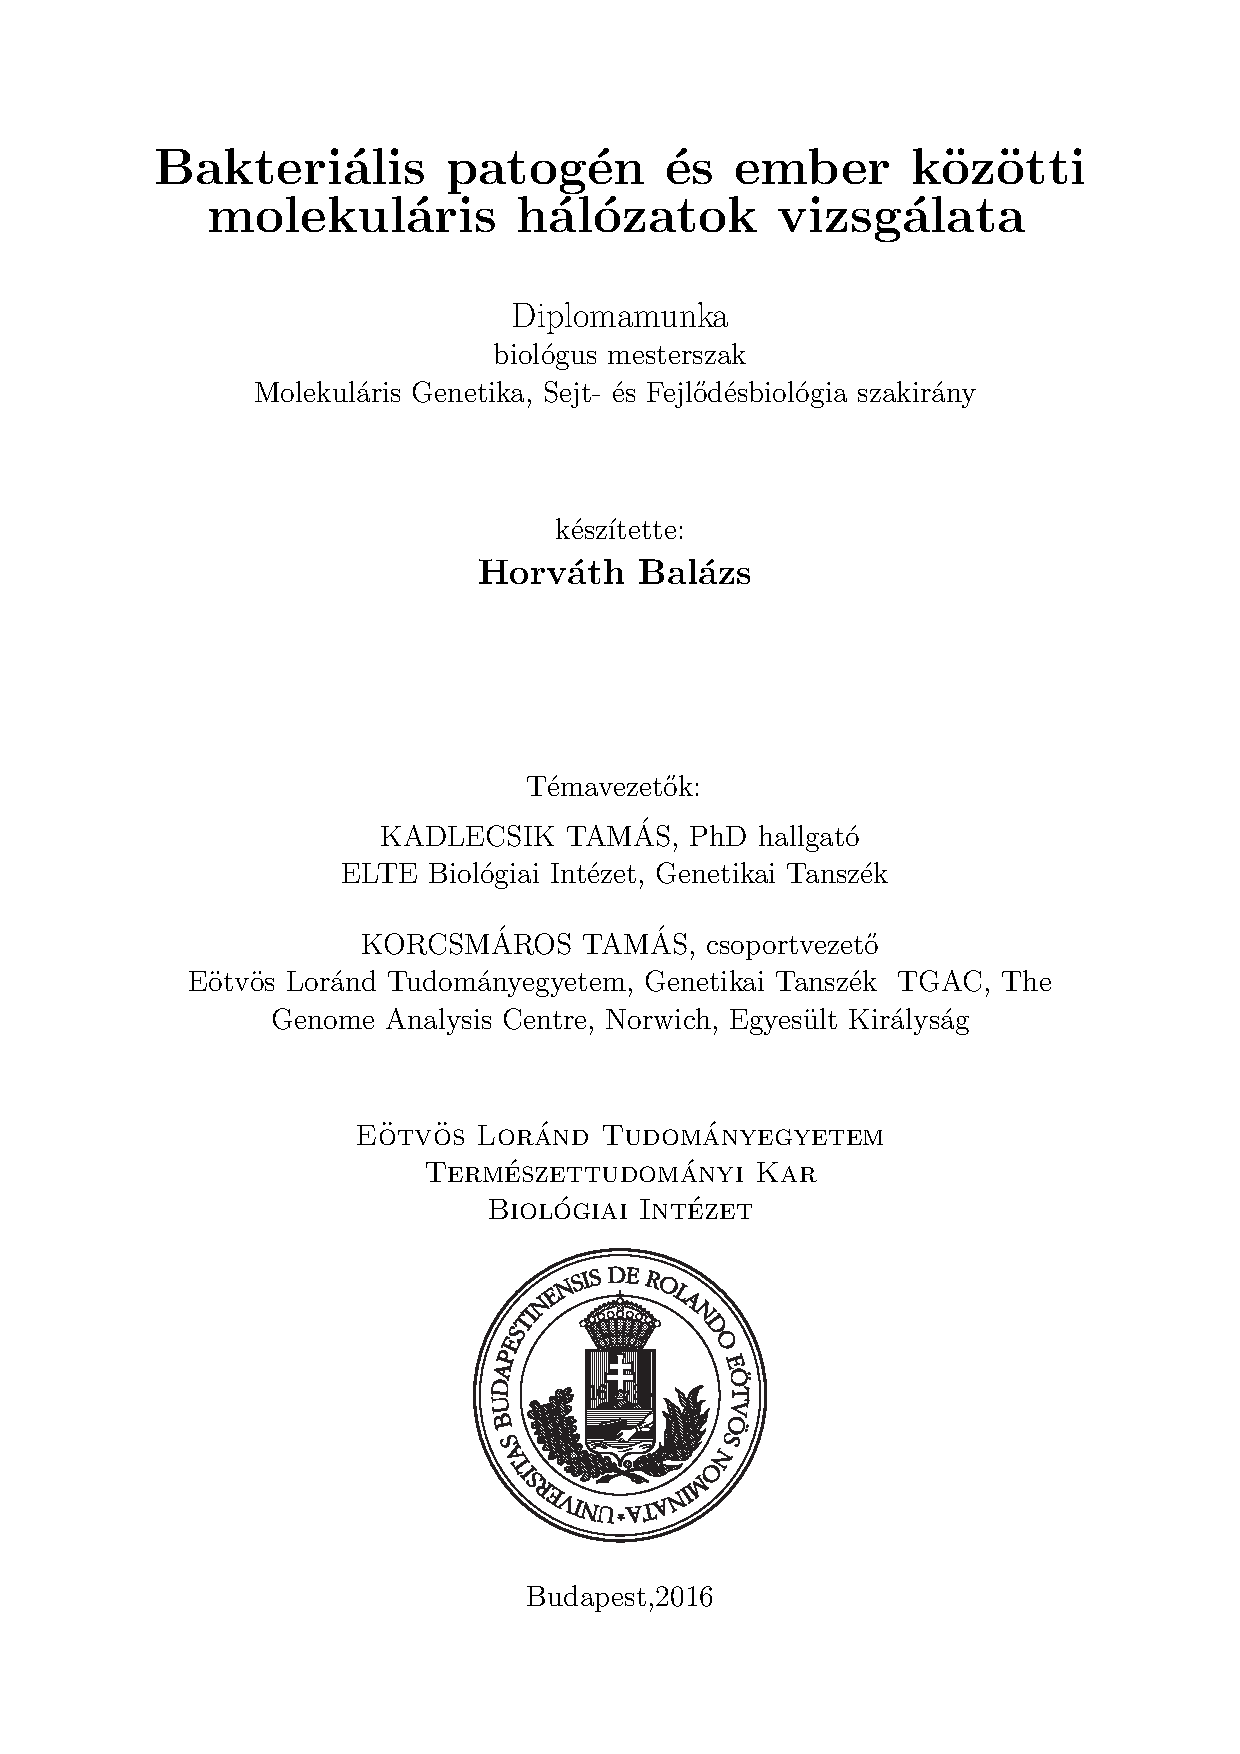
\includepdf[pages={1}]{cimlap.pdf}

\pagebreak

% tartalomjegyzék
\setcounter{page}{1}
\tableofcontents


\pagebreak

\section{Rövidítésjegyzék}

		
		\begin{table}[H]
		\centering
		\resizebox{\columnwidth}{!}{
		\begin{tabular}{rlrl}
		\textit{\textbf{Rövidítés}} & \textit{\textbf{Magyarázat}}                                                                        & \textit{\textbf{Rövidítés}} & \textit{\textbf{Magyarázat}}                                                                              \\
		ATG                         & \begin{tabular}[c]{@{}l@{}}Autofágiával kapcsolatos gének \\ (Autophagy-related genes)\end{tabular} & NCBI                        & \begin{tabular}[c]{@{}l@{}}National Center for \\ Biotechnology Information\end{tabular}                  \\
		BC                          & Betweenness Centrality                                                                              & NBR1                        & Next to BRCA1                                                                                             \\
		BECN1                       & Beclin-1                                                                                            & NDP52                       & nuclear dot protein 52 kDa                                                                                \\
		CC                          & Closeness Centrality                                                                                & OPTN                        & Optineurin                                                                                                \\
		E1                          & Ubikvitin aktiváló enzimek                                                                          & p62 (SQSTM1)                & \begin{tabular}[c]{@{}l@{}}ubikvitin-kötő fehérje \\ p62, Sequestosome-1\end{tabular}                     \\
		E2                          & Ubikvitin konjugáló enzimek                                                                         & PI3K                        & \begin{tabular}[c]{@{}l@{}}foszfatidilinozitol-\\ 4,5-biszfosfát 3-kináz\end{tabular}                     \\
		E3                          & Ubikvitin ligáz                                                                                     & PPI                         & fehérje-fehérje kapcsolat                                                                                 \\
		GABARAP                     & \begin{tabular}[c]{@{}l@{}}Gamma-aminobutyric acid \\ receptor-associated protein\end{tabular}      & PSI                         & Proteomics Standards Initiative                                                                           \\
		GPCR                        & \begin{tabular}[c]{@{}l@{}}G-fehérje kapcsolt receptor\\ (G-protein coupled receptor)\end{tabular}  & SCFA                        & \begin{tabular}[c]{@{}l@{}}rövid láncú zsírsav \\ (Short Chaine Fatty Acid)\end{tabular}                  \\
		GPRs                        & \begin{tabular}[c]{@{}l@{}}Rövidlánci zsírsav receptorok \\ (Free fatty acid receptor)\end{tabular} & SCV                         & Salmonella Containing Vacoule                                                                             \\
		IBD                         & \begin{tabular}[c]{@{}l@{}}gyulladásos bélbetegség\\  (Inflammatory Bowel Disease)\end{tabular}     & SIF                         & \begin{tabular}[c]{@{}l@{}}Salmonella által \\ kiváltott filamentumok\end{tabular}                        \\
		IFR                         & Institute of Food Research                                                                          & SPI-I és II                 & \begin{tabular}[c]{@{}l@{}}Salmonella patogenitási\\ sziget 1 és 2\end{tabular}                           \\
		LC3                         & light chain 3 (ATG8 homológ)                                                                        & SQL                         & Structured Query Language                                                                                 \\
		MAP                         & Microtubule Associated Protein                                                                      & T3SS                        & \begin{tabular}[c]{@{}l@{}}Hármas típusó szekréciós rendszer\\ (Type three secretion system)\end{tabular} \\
		mTORC1                      & \begin{tabular}[c]{@{}l@{}}mammalian target of\\  rapamycin complex 1\end{tabular}                  & TrEMBL                      & \begin{tabular}[c]{@{}l@{}}Translated EMBL Nucleotide\\  Sequence Data Library\end{tabular}              
		\end{tabular}}
		\end{table}
		
		
		\pagebreak

\section{Bevezetés}
	\subsection{A bél mikrobióta fontosságának ismertetése}
		\paragraph{Miért van szükség a bél mikrobióta vizsgálatára?} \mbox{}\\
		A humán bél mikrobióta egy komplex ökoszisztéma. A mikrobiomot alkotó sejtek száma nagyjából a humán szomatikus és csírasejtek összegének tízszerese \cite{scfa_and_vitamine}.  A bél mikrobiom mind metabolikusan, mind immunológiailag komplex kapcsolatban áll az emberrel \cite{gut_microbiome}. Az emberi béltraktusban eddig több mint három millió nem redundáns mikrobiális gént sikerült kimutatni \cite{meta_omics}. Ez a nagy genetikai állomány lehetővé teszi, hogy olyan metabolikus folyamatok játszódjanak le az emberi bélben, melyeket az sejtjeink nem képesek végrehajtani \cite{gut_microbiome}. A bél mikrobióta felelős bizonyos glikánok, aminosavak és xenobiotikumok metabolizmusáért valamint rövid láncú zsírsavak (\textit{short chained fatty acids - SCFA}-k), vitaminok és kofaktorok termeléséért. A gazda által meg nem emésztett poliszacharidok bontását is a bél mikrobióta végzi. Ez utóbbi folyamat eredményeképpen olyan rövid láncú zsírsavak keletkeznek mint az acetát, proprionát és vajsav \cite{scfa_and_vitamine}.
		
		A bélflóra kulcsszerepet játszik az immun-homeosztázis fenntartásában. A mikrobióta az immunrendszerrel bakteriális mintázatokat észlelő receptorokon és G-fehérje kapcsolt receptorokon (GPCR) keresztül van kapcsolatban. A mikroorganizmusok által termelt SCFA-k képesek GPCR-eken révén a sejtszignalizáció indítására. Például a veleszületett immunrendszer nagy részét alkotó monociták és neutrofil granulociták rendelkeznek GPR43 receptorral. A GPR43 egy SCFA érzékeny receptor. Tehát az immunrendszer a patogén mintázatot felismerő receptorok mellett, a metabolitokra érzékeny GPR43-on keresztül is kapcsolatban a bélflórával \cite{buthyrate_immune}.
		
		A bélflóra hatással van még a gazda metabolizmusára is.  Az \textit{Eubacterium spp.} által oligoszacharidokból képzett vajsav részt vesz az emberi szervezet energia egyensúlyának szabályzásában \cite{gut_microbiome}. Az enteroendokrin sejtek és az adipociták is rendelkeznek GPR41 receptorral mely vajsavra és proprionátra is érzékeny. Adipocitáknál ez a GPR41 szignalizáció \textit{leptin} elválasztást eredményez \cite{buthyrate_immune}. A vajsav segít a karcinogenezis kivédésében mivel apoptózis indukáló és proliferáció gátló hatása van. Éppen ezen okokból a bél mikrobióta tekinthető egy új metabolikus szervnek is\cite{scfa_and_vitamine}. Kapcsolatok mutathatók ki a bél mikrobiom megváltozása és olyan betegségek között mint az IBD (\textit{inflammatory bowl disease}), elhízás vagy a különböző rák típusok \cite{gut_microbiome}.
		
		\paragraph{A bél mikrobióta vizsgálatának módszerei} \mbox{}\\
		A mikrobióta vizsgálatát elsősorban a különböző meta-omikák eszköztárával közelítik meg. Ezek közül is a legfontosabb eszköztár a metagenomika, de alkalmaznak már metabolomikai, metatranszkriptomikai és metaproteomikai megközelítést is. A metagenomikai vizsgálatok során a környezetből származó mintát megfelelő előkészítés után közvetlenül \textit{shotgun} szekvenálásnak vetik alá \cite{gut_microbiome}.
		
		Quin és társai 2010-re meghatározták a minimális bél metagenomot. A vizsgálat során \textit{Illumina GA short-read} alapú technológiával 124 egy kohortba tartozó nordikus és mediterrán személy székletmintáját elemezték. Az ebből kinyert 576,7 gigabázásnyi DNS-ből mintegy 3,3 millió nem redundáns mikrobiális gént mutattak ki. Az így kimutatott gének az emberi genom százötvenszeresét teszik ki. A minták egészére jellemző, hogy a bennük található gének két fő részre osztható: A legnagyobb csoportba (86\%) a sűrűn előforduló mikrobiális gének, míg a másik fő csoportba a kifejezetten a humán bélflórára jellemző mikrobiális gének tartoznak. Az összes személyből származó vizsgált génhalmaz 99,1\%-a \textit{Eubacteria}, 0,8\%-a \textit{Archea} és a fennmaradó 0,1\%-a pedig vegyesen \textit{Eucaryota} és virális eredetű. A bakteriális eredetű gének összesen 1000-1150 uralkodó baktériumfajhoz tartozhatnak, ami személyenként kb. 160 domináns fajt jelent. A személyekre jellemző nagyjából 160 uralkodó baktériumfaj listái között a személyeket összevetve nagyfokú hasonlóság figyelhető meg. Egy adott személy bél metagenomjának minimálisan 40\%-a megtalálható a minták legalább felében. A közelítőleg ezer fajból 75 faj található meg a minták több mint felében és 57 faj van ami a minták nagyobb mint 90\%-ban kimutatható  \cite{meta_omics}.
		
	
	\subsection{A Humán-\textit{Salmonella} kapcsolat ismertetése és hatása az autofágiára}
	
		\paragraph{\textit{Salmonella spp.}} \mbox{}\\
		A \textit{Salmonella} olyan Gram-negatív patogén mely az állatok széles skáláját képes fertőzni. A tudomány jelenleg több ezer szerotípust ismer, melyek két fő kategóriára oszthatók. Az egyik fő típus a \textit{Typhoid}, ebbe a csoportba tartozik a \textit{Typhi} és \textit{Paratyphi} melyek kifejezetten embert fertőznek. A másik fő csoport a \textit{Non-typhoid} amelybe tartozó baktériumok már széleskörű gazdaspecificitással rendelkeznek \cite{salmonella_and_host_cell_nature}.
		
		A fertőzés kontaminált étel vagy folyadék fogyaztásával történik. A \textit{Salmonella} az alacsony pH és oxidatív stressz ellen adaptív toleranciával rendelkezik, így képes eltűrni a gyomor savasságát és a veleszületett immunrendszer egyéb hatásait. A vékonybélbe jutva az epithélium sejtjeit fertőzik. Fő célpontjaik a \textit{microfold} (\textit{M cells}) sejtek, melyek fő feladata, hogy pinocitózissal mintákat vegyenek a középbél tartalmából. Amennyiben a felvett anyag károsnak bizonyul, azt antigén prezentáló sejtekhez juttatják \cite{salmonella_and_host_cell_nature}. A \textit{Salmonella} másik célpontja a nem fagocita típusú enterociták. Ezekbe a sejtekbe úgynevezett baktérium-közvetített endocitózissal képesek bejutni \cite{salmonella_and_host_cell_nature}.
		
		
		\paragraph{A \textit{Salmonella} életciklusa} \mbox{}\\
		Az intracelluláris baktériumok életciklusa általánosan három stádiumra osztható: A bejutáshoz használt vakólum elhagyása, replikáció a citoszólban és a citoszólikus veleszületett immunitás elemeinek manipulációja. A \textit{Salmonella} az úgynevezett \textit{trigger} mechanizmussal jut be a sejtbe. A mechanizmus során a baktérium olyan fehérjéket juttat be az eukarióta sejtbe, melyek képesek a sejtvázzal kölcsönhatni. Ezek a bakteriális effektorfehérjék nagyfokú sejtváz-átrendeződést váltanak ki az eukarióta gazdában. A folyamat végén a baktérium egy vakólummal határolva a sejt belsejébe kerül \cite{salmonella_autophagy_nature_old}. Ezt a struktúrát a szakirodalomban SCV-nek nevezik (\textit{Salmonella containing vacuole}) \cite{salmonella_and_host_cell_nature}.
		
		A fagocitózis végeztével a \textit{Salmonella} átesik egy úgynevezett bakteriális felszín átformázáson (\textit{bacterial surface remodeling}). A folyamat során gátlódik az olyan bakteriális gének kifejeződése amelyeket a gazda könnyen fertőzési jelnek tekinthet. Ilyen gének például a SPI1, a T3SS és a flagellin. Mindezek mellett megváltozik a baktériumok felszíni lipopoliszacharid mintázata is  \cite{salmonella_and_host_cell_nature}.
		
		 \begin{figure}[H]
			 \centering
			 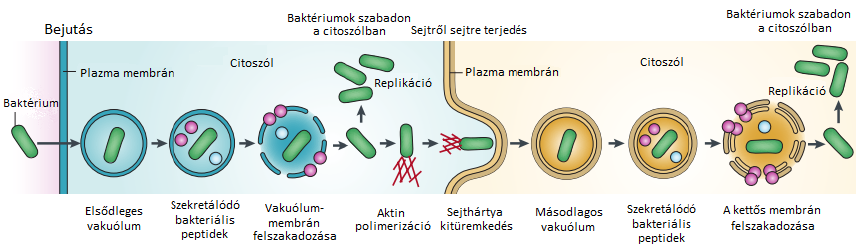
\includegraphics[scale=0.7]{img/intracell_bakt_terj_am.png}
			 \caption{\textbf{Az intracelluláris baktériumok életciklusa}}
			 \begin{imgdesc}
				 Bejutáskor a baktériumok egy elsődleges vakólumba érkeznek. A sejt a belsejében a mikróbák olyan fehérjéket szekretálnak, melyek felbontják az őket határoló elsődleges vakólum membránját. A legtöbb intracelluláris baktériumra jellemző, hogy befolyásolni tudja az aktin polimerizációt és ezáltal képes az intra- és intercelluláris mozgásra. A szomszédos sejtbe átjutott baktériumok egy másdlagos memránburokba kerülnek, melyet ugyancsak felbontanak.
			 \end{imgdesc}
			 \label{fig:salmo_cycle}
		 \end{figure}
		
		 Normális körülmények között a vakólum pH-ja mindaddig fokozatosan csökken amíg érett degradatív fagolizoszómává nem válik. A baktériumok kétféleképpen képesek életben maradni ebben a környezetben: A vakólum-lizoszóma fúzió gátlásával, vagy a fagolizoszóma összetételének aktív módosításával \cite{salmonella_autophagy_nature_old}. A szakirodalomban még nincs kialakult álláspont arról, hogy a \textit{Salmonella} melyik mechanizmust használják. Bizonyítottan képesek életben maradni, olyan SCV-ben mely már fuzionált a lizoszómával, viszont a fő útvonal valószínűleg a vakólum savanyítási folyamatának késleltetése lehet \cite{salmonella_and_host_cell_nature}. 
		 
		 Az SCV-n belül a \textit{S.} Typhimurium képes a replikációra. A hármas típusú szekréciós rendszer segítségével a baktériumsejtek olyan anyagokat tudnak kibocsájtani, melyek lehetővé teszik az SCV-ből kijutást és citoplazma invázióját \cite{salmonella_authopagy_intro}.
		 
		 \paragraph{A hármas típusú szekréciós rendszer (T3SS vagy TTSS)} \mbox{}\\
		 A T3SS evolúciósan a flagelláris export rendszerrel mutat rokonságot. Jelenléte esszenciális ahhoz, hogy a \textit{Salmonella} képes legyen a fertőzésre és gazda sejtjeinek kolonizálására. A T3SS felelős a baktérium virulencia vagy effektor fehérjéinek átviteléért. Az effektorok az eukarióta sejtbe jutva megváltoztatják annak sejtfunkcióit. Az virulenciafehérjék átalakítják a gazda citoszkeleton architektúráját, membrán anyagáramlását, szignál transzdukcióját és citokin expresszióját, ezzel segítve a baktériumok túlélését és további kolonizációját \cite{salmonella_and_host_cell_nature}.
		 
		 \paragraph{A \textit{Salmonella} és az autofágia kapcsolata} \mbox{}\\
		 Az autofágia egy intracelluláris katabolikus folyamat melynek szerepe van a fehérje aggregátumok és károsodott sejtorganellumok eltávolításában és a veleszületett immunrendszer működésében. A \textit{xenofágia} az autofágiának azon formája mely során az intracelluláris baktériumok és vírusok szelektív felismerése és lebontása történik. A szelektív felismerésért az autofágia adaptor fehérjéi felelősek. Ilyen receptor fehérje például a p62 (SQSTM1), a NDP52, optineurin (OPTN) és az NBR1. Az előbb felsorolt receptorok a szubsztrátjuk megkötése után kargo adaptorként viselkednek az LC3 (ATG8) számára. \textit{Salmonella fertőzéskor} a sérült SCV-ből kilépett baktériumok sejtfelszíni fehérjéi poliubiquitin borítást kapnak amit a kargo adaptor fehérjék érzékelnek. \textit{S.} Typhimurium fertőzéskor a poliubiquitinált baktériumokat NDP52 és a p62 is felismeri. Az így megkötött baktériumok xenofágia útján eltávolítódnak \cite{salmonella_authopagy_intro}.
	
	\subsection{Ökológiai hálózatok elemzésére használt topológiai indexek}
	
	 \paragraph{Az ökológiai mérőszámok}
	 Első ránézésre egy gazda és patogén baktérium kapcsolata valamint a szupraindividuális rendszereket jellemző mérőszámok egy helyen tárgyalása különlegesnek tűnhet. Jobban belegondolva, viszont e két rendszer sok hasonlóságot mutat egymással, ugyanis mindkettő modellezhető hálózatként. Hálózatok topológiai jellemzését eleinte a szociológiában majd később az ökológiában kezdték alkalmazni \cite{top_indexes}. A molekuláris hálózatok leírására még elég ritkán alkalmaznak tisztán topológiai mérőszámokat. Diplomamunkám során egy gazda-patogén molekuláris hálózatot fogok ökológiai eredetű tisztán topológiai mérőszámmal jellemezni. 
	 
	 \paragraph{Miért van szükség topológiai mérőszámokra?} \mbox{}\\ %linebreak after paragraph title
	 A konzervációbiológia az élettudományok azon ága mely a Föld biodiverzitásának megőrzésével foglalkozik. Mivel az összes faj védelme nem megoldható, ezért szükségessé vált olyan fajok kiválogatása melyek kiemelt figyelmet igényelnek konzervációs biológiai szempontból\cite{new_zeland}. Az 1990-es évek előtt a védelemre való kiválasztás fő szempontja a faj ritkasága volt.  A fajok ilyen alapú szelekciója nem veszi figyelembe hogy például az adott taxon kulcsszerepet játszik-e az ökoszisztéma funkciók ellátásában \cite{jordan_comparison}.
	 
	 \paragraph{Kulcsfajok} \mbox{}\\ %linebreak after paragraph title
	 1966-ban Robert Paine megalkotta a kulcsfaj koncepciót (\textit{keystone species}). Megfigyelte hogy ha kiesik a Kaliforniai sziklás tengerparti közösségből a \textit{Piaster ochraceus} csúcsragadozó tengeri csillag akkor az egész közösség fajösszetétele összeomlik. A mai legelfogadottabb kulcsfaj definíció szerint ezek olyan fajok, melyek ökológiai hatása aránytalanul nagy az abundanciájukhoz képest. A fogalommal kapcsolatban azonban további kérdések merülnek fel: Milyen hatás számít nagynak? Pontosan mekkora biomassza hányad után mondható az adott faj ereje aránytalannak \cite{new_zeland}? Ez utóbbi kérdések megválaszolásához szükség van olyan mérőszámokra, melyek segítségével kvantitatívvé tehető egy adott faj ökológiai fontossága. Másrészt így lehetővé válik a fajkiválasztás során fellépő szubjektivitás csökkentése. Az ilyen mérőszámok használatával objektív fontossági sorrendet lehet felállítani az adott élőhelyen előforduló taxonok között \cite{jordan_comparison}.
	 
	 \paragraph{Rangsorolásra használt topológiai mérőszámok az ökológiában} \mbox{}\\
	 Ma már a kulcsfajok kiválasztása részben ökológiai interakciós hálózatok elemzése alapján történik. A használt hálók kizárólag biotikus-biotikus (faj-faj) kapcsolatokat tartalmaznak. Erre azért van szükség, mert például minden élőlény összekötésben áll a detritusszal és ez eltorzítaná az analízis eredményét. Sőt ilyen esetben a detritusz maga is struktúrális kulcsfajnak számítana. Egy adott fajnak az ökológiai interakciós hálóban betöltött szerepét pozicionális fontossági mérőszámokkal, vagy más néven centralitási indexekkel lehet jellemezni. A konzervációs biológiában sokfajta ilyen mérőszámot használnak, melyeknek közös tulajdonsága, hogy mindegyik valamilyen egyedi tulajdonságra fekteti a hangsúlyt és az alapján rangsorolja a hálózatban szereplő fajokat. Ilyen eltérés lehet két index között például, az hogy az egyik egy adott pont lokális kapcsolati mintázatára, míg a másik az egész hálózatra vonatkozó hatását számszerűsíti. Adott hálóra különböző mérőszámok eltérő fajsorrendeket adnak, de a hasonló tulajdonságok figyelembevételén alapuló mérőszámok között felállíthatók konszenzus fák \cite{jordan_comparison}.
	 
	 \paragraph{Főbb topológiai mérőszámok} \mbox{}\\
	 A bonyolult rendszereket modellező hálózatok topológiája alapján sok fontos információ nyerhető a rendszer működéséről. A következő néhány bekezdésben a hálózattudományban alkalmazott legfontosabb mérőszámokat szeretném röviden ismertetni. Végül egy részletesebb leírásban a diplomamunkám alapjául szolgáló TI-t mutatom be.
	 
	 \paragraph{Normalised degree - D} \mbox{}\\Az adott ponttal kapcsolódó pontok száma elosztva a hálózat összes pontjának számával \cite{top_indexes}.
	 
	 \paragraph{Closeness centrality - CC vagy C } \mbox{}\\ A pontok száma elosztva az adott pontból eredő azt minden más ponttal összekötő legrövidebb topológiai távolságok összegével \cite{top_indexes}. Ez a mérőszám megmutatja, hogy egy adott pontnak mekkora az átlagos távolsága a hálózat összes többi pontjától. Az index kicsi szám olyan pontokra melyek rövid legrövidebb útvonalakon vannak a többi ponttal összekötve. Az ilyen pontok valószínűleg könnyebben elérnek más pontokat vagy nagyobb hatást tudnak gyakorolni más pontokra. Adott $i$ pont átlagos legrövidebb távolságát a többi ponttól a következőképpen lehet kiszámolni \cite{newman_networks}:
	 
	 	\begin{equation}
			\ell_i= \frac{1}{n-1} \sum_{j} d_{ij} \qquad \mathrm{vagy,} \qquad \ell_i= \frac{1}{n} \sum_{j (\neq i)} d_{ij}
	 	\end{equation}
	 	 \noindent{Ahol}:
	 	 \begin{itemize}[label=]
	 	 	\item $\ell_i$ : Az $i$ pont átlagos legrövidebb távolsága a hálózat többi pontjától.
			\item $d_{ij}$ : Az az i pontot a j ponttal összekötő legrövidebb útvonal (geodézikus útvonal) pontjainak száma.
			\item $n$: A hálózat pontjainak száma.
	 	 \end{itemize}
	 
	 A két számítás között stratégiai különbség van. A baloldali egyenlet azt feltételezi, hogy adott pontnak önmagára mért hatása nem releváns a hálózat működésének szempontjából. Azonban még erre az esetre is jellemző, hogy mivel definíció szerint a $d_{ii}$ távolság 0, ezért az összeget ez az érték nem növeli csupán az osztót \cite{newman_networks}.  \\
	 Az $\ell_i$ érték önmagában még nem centralitási index, mert kis számokat ad a magas központiságú pontokra. Ahhoz, hogy megkapjuk a \textit{Closeness Centrality}-t az $\ell_i$ inverzét kell vennünk \cite{newman_networks}:
	 
	 	\begin{equation}
			C_i = \frac{1}{\ell_i}
	 	\end{equation}
	 
	 \paragraph{Betweenness centrality - BC} \mbox{}\\ 
	 A vizsgálni kívánt ponton áthaladó a hálózat többi pontpárját összekötő legrövidebb utak összege elosztva a hálózat többi pontpárját összekötő összes legrövidebb út összegével \cite{top_indexes}. 	 Ez a mérőszám azt mutatja meg, hogy egy adott pont milyen arányban szerepel a többi pont között futó útvonalakon. A \textit{betweenness centrality} vagy röviden  \textit{betweenness} olyan hálózatok jó jellemzője, melyekben valamilyen természetű ``áramlás" folyik a pontok között. Ha feltételezzük, hogy egy ilyen hálózat minden kapcsolata között az áramlás során ugyanannyi kicserélődés történik egy egységnyi idő alatt és a kicserélődés a legrövidebb útvonalakon folyik, akkor az összes geodézikus útvonalon is azonos rátával történik az áramlás. Ez azt jelenti, hogy egy adott ponton átmenő áramlás mennyisége arányos azzal, hogy a hálózat legrövidebb útvonalainak milyen arányában szerepel \cite{newman_networks}.
	 
	 \paragraph{Topological importance - TI\textsuperscript{n}}  \mbox{}\\
	 A diplomamunkám során ezt a mérőszámot alkalmazom az általam összeállított molekuláris hálózatokra. Ezen okból a következő néhány bekezdésben, egy jóval részletesebb leírásban mutatom be a TI kiszámításának módját és mérőszám tulajdonságait. 
	 
	 Ez egy teljesen topológiai alapú mérőszám mely összegzi az egy adott pontból kiinduló összes lehetséges \textit{n} lépéshosszúságú útvonal hatását. A hálózat összes direkt kapcsolatára kiszámítható azok topológiai erőssége:
	 
	 \begin{equation}
		d_{X,Y} = \frac{1}{x}
	 \end{equation}
	 
 	 \noindent{Ahol}:
 	 \begin{itemize}[label=]
		 \item $d_{X,Y}$ : Az Y pont hatása X pontra.
		 \item $x$ : Az X pont első szomszédainak száma.
 	 \end{itemize}
	 
	 Az így kiszámolt közvetlen kapcsolatok hatását egy mátrixban lehet ábrázolni, melynek indexelése a populációdinamika konvencióit követi: \textit{d}\textsubscript{\textit{ij}} jelenti a \textit{j} pontnak az \textit{i} pontra gyakorolt hatását. Adott direkt kapcsolat hatásának nagysága a kapcsolat irányától is függ, tehát \textit{d}\textsubscript{\textit{ij}} nem feltétlenül ugyanakkora mint \textit{d}\textsubscript{\textit{ji}}. Egy \textit{n} lépés hosszú útvonal erejét az ezt alkotó direkt kapcsolatok hatásának szorzataként értelmezzük:
	 
	 \begin{equation}
		d^n_{p_{XY}} =\prod_{i=1}^{n-1} d^1_{i, i+1} 
	 \end{equation}
	 
	 
	 \noindent{Ahol}:
	 \begin{itemize}[label=]
		 \item $p_{XY}$: Útvonal amire igaz hogy $p \in$ \{$X$ és $Y$ közötti $n$ lépés hosszúságú útvonalak\}
		 \item $d^n_{p_{XY}}$: Az $X$ és $Y$ pontok közötti $n$ lépés hosszú $p$ útvonal ereje.
		 \item $d^1_{n, n+1}$: Az útvonal $i$ és $i+1$-ik pontja közötti direkt kapcsolat erőssége
	 \end{itemize}
	 
	  \noindent{Ez alapján egy $Y$ pont hatása $X$-ra $n$ lépés távolságban:}
	 
	 \begin{equation}
		 d^n_{XY} = \sum d^{n}_{p_{XY}}
	 \end{equation}
	 \noindent{Ahol}:
	 \begin{itemize}[label=]
		\item $p_{XY}$: Útvonal amire igaz hogy $p \in$ \{$X$ és $Y$ közötti $n$ lépés hosszúságú útvonalak\}
		\item $d^n_{XY}$: Az összes $Y$ pontból eredő és $X$-ben végződő $n$ hosszúságú útvonalak erejének összege. 
	 \end{itemize}	 
	 
	 Mivel a direkt kapcsolatok ereje függ a kapcsolat irányától, így a TI tükrözi a kapcsolat asszimmetrikusságát is. Egy adott pontra TI\textsuperscript{n} a következő képen számítható ki:
	 
	 \begin{equation}
		\textrm{TI}^n_A=\sum d^n_{j,A}
	 \end{equation}
	 
	 \noindent{Ahol}:
	 \begin{itemize}[label=]
		 \item  $\textrm{TI}^n_A$: $A$ pont $n$ lépésre számított topológiai fontossága.
		 \item  $d_{j,A}$: $A$ és $j$ pont közötti $n$ hosszúságú útvonalak ereje. 
	 \end{itemize}
	 
	A TI$^n$-t a hálózat összes pontjára ki lehet számítani és ez alapján sorrendet lehet felállítani a nódusok között.
	 
 	 \begin{figure}[H]
 		 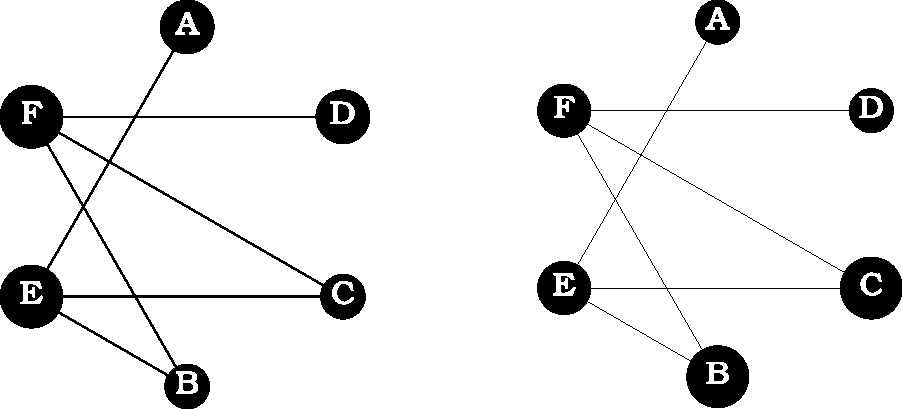
\includegraphics[scale=1]{img/graphs.pdf}
 		 \centering
 		 \caption{\textbf{TI$^1$ \textit{(bal)} és TI\textsuperscript{2} \textit{(jobb)} szemléltetése ugyanazon a példagráfon} }
 		 A pontok átmérője arányos az adott nódusra kiszámolt TI$^1$ \textit{(bal)} és TI$^2$ (\textit{jobb)}). (\cite{ti}) alapján módosítva.
 		 \label{fig:peldagraph}
 	 \end{figure}
 	 
 	 A \ref{fig:peldagraph}. ábrán látható példagráfra rendre felírhatóak a közvetlen  kölcsönhatások ($d$) és a két lépésnyire közvetített indirekt kölcsönhatások ($d^2$) értékeit tartalmazó mátrixok:
	
	% Példamátrixok %
	\[
	\begin{blockarray}{ccccccc}
	&A & B & C & D & E & F \\
	\begin{block}{c [cccccc]}
	A &0 & 0 & 0 & 0 & \frac{1}{3} & 0 \\[6pt] 
	B & 0 & 0 & 0 & 0 & \frac{1}{3} & \frac{1}{3}\\[6pt] 
	C & 0 & 0 & 0 & 0 & \frac{1}{3} & \frac{1}{3}\\[6pt] 
	D & 0 & 0 & 0 & 0 & 0 & \frac{1}{3}\\[6pt] 
	E & 1 & \frac{1}{2} & \frac{1}{2} & 0 & 0 & 0\\ [6pt] 
	F & 0 & \frac{1}{2} & \frac{1}{2} & 1 & 0 & 0\\ [6pt]
	\end{block}
	\multicolumn{7}{c}{\indent $d$ értékek} \\ [6pt]
	\end{blockarray},\quad
	\begin{blockarray}{ccccccc}
	&A & B & C & D & E & F \\ 
	\begin{block}{c [cccccc]}
	A & \frac{1}{3} & \frac{1}{6} & \frac{1}{6} & 0 & 0 & 0 \\[6pt] 
	B & \frac{1}{3} & \frac{1}{3} & \frac{1}{3} & \frac{1}{3} & 0 & 0\\ [6pt] 
	C & \frac{1}{3} & \frac{1}{3} & \frac{1}{3} & \frac{1}{3} & 0 & 0\\[6pt] 
	D & 0 & \frac{1}{6} & \frac{1}{6} & \frac{1}{3} & 0 & 0\\[6pt] 
	E & 0 & 0 & 0 & 0 & \frac{2}{3} & \frac{1}{3}\\ [6pt] 
	F & 0 & 0 & 0 & 0 & \frac{1}{3} & \frac{2}{3}\\ [6pt]
	\end{block}
	\multicolumn{7}{c}{\indent $d^2$ értékek} \\[6pt]
	\end{blockarray}
	\]
	
	Az ábrázolt mátrixok elrendezése követi a populációdinamikai konvenciókat, tehát például $d_{BF}=\frac{1}{2}$ azt jelenti, hogy $F$ pont a $B$-re $\frac{1}{2}$ erővel hat. Mindkét mátrixra érvényes az, hogy az adott oszlop értékeinek összege egy. Ez a tulajdonság a $d$ érték definíciójából fakad. $d$ azt mutatja meg, hogy adott pont a cél pont kapcsolatainak hányad részét adja. Ezáltal minden pont egy egységnyi hatást kap ami eloszlik a vele kapcsolatban álló pontok között (\cite{ti}). Ezt a hatást jól szemlélteti a \ref{fig:peldagraph}. ábra bal oldali része amin látható, hogy az $A$, $B$, $C$ és $D$ pontok kimenő hatása kisebb, mivel célpontjaik sok hatást fogadnak.
	
	Ugyancsak mindkét mátrixra jellemző, hogy a sorok összege azt mutatja meg, hogy egy adott pont mennyire erős kölcsönható, tehát mekkora TI$^n$ értéke. Például $B$ pont két lépés távolságban összesen $\frac{4}{3}$ erővel hat, ez alapján erősebb kölcsönhatónak mondható mint az $A$ pont a maga $\frac{2}{3}$ értékű összesített kimenő két lépés hosszú hatásaival (\cite{ti}).
	
	Az \ref{fig:peldagraph}. ábrán az is jól megfigyelhető, hogy $C$ pont a gyengébb közvetlen kölcsönhatók közé tartozik. Ugyanakkor mivel a $C$-ből eredő két lépéses útvonalak erős elsődleges kölcsönhatókon keresztül érik el végpontjaikat, ezáltal két lépés távolság viszonylatában már $C$ is az erős kölcsönhatók közé tartozik. \\
	\indent Az $n > 1$ lépésszámú $d^n$ értékeket tartalmazó mátrixokban már egy adott pont indirekt hatása önmagára is kiterjedhet. Páros számú lépések esetén viszont mindenképpen felírhatók olyan útvonalak melyeken a pont eléri önmagát, (\cite{ti}) vagyis $d^n_{X,X} \neq 0$ ha n $\in$ \{ $2k :  k \in \mathbb{Z}$ \}. Az \ref{fig:peldagraph}. ábrán látszik, hogy például az $F$ pont két lépés távolságban a következű útvonalakon hat önmagára: $F \rightarrow B \rightarrow F$, $F \rightarrow C \rightarrow F$ és  $F \rightarrow D \rightarrow F$.
 	 \pagebreak

\section{Célkitűzések}
	\paragraph{A diplomamunka célja} \mbox{}\\
	A diplomamunkám célja egy több adatbázisból integrált fehérje-fehérje kapcsolatokat tartalmazó humán-\textit{Salmonella} gazda-patogén hálózat létrehozása és az így elkészült hálózat topológiai elemzése.
	
	
	Az elkészítendő hálózatnak a következőket kell tartalmaznia:  
	\begin{enumerate}
			\item kézzel gyűjtött  \textit{H. sapiens} fehérje-fehérje kapcsolatok
			\item kézzel gyűjtött  \textit{Salmonella} fehérje-fehérje kapcsolatok
			\item \textit{H. sapiens} és \textit{Salmonella} közti prediktált fehérje-fehérje kapcsolatok
	\end{enumerate}
	
	A topológiai elemzés során kapott adatok alapján véleményt szeretnék alkotni arról, hogy felhasználhatók-e az ökológiában fajok közti kapcsolatok vizsgálatára használt tisztán topológiai adatokon alapuló mérőszámok a molekuláris kapcsolati hálók elemzésére. Valamint, hogy az így előállított rangsorok mennyire korrelálnak a jelenleg használt \textit{Salmonella} és humán bélsejteket vizsgáló módszerek eredményeivel.

	\paragraph{A célok eléréséhez tervezett feladatok}
	\begin{enumerate}
		\item Olyan adatszerkezetek és keretrendszer fejlesztése mely képes molekuláris hálózatok feldolgozására.
		\item Az \textit{ARN} a \textit{Salmonet} és az  ember-\textit{Salmonella} predikciók alapján integrált gazda-patogén hálózat készítése.
		\item A TI mérőszámot kiszámolni képes program fejlesztése és, annak tesztelése hogy a TI alkalmas-e kifejezetten a gazda-patogén molekuláris hálózatok leírására.
	\end{enumerate}
	\pagebreak

\section{Források és módszertan}

	\subsection{Informatikai módszerek}
			\paragraph{A problémák megoldására használt programnyelvek} \mbox{}\\
			A teljes adatbázisok feldolgozására valamint az adatbázisokból származó adatok rendszerezésére és megfelelő formátumúra alakítására \textit{Python} programnyelven írtam szkripteket. A diplomamunkám során a \textit{Python} 2.7-en és 3.4-en futtatható szkripteket alkalmaztam. A fehérjék azonosítójának fordítását végző szkriptek egyike témavezetőm Kadlecsik Tamás \textit{Javascript}ben írt fordítószkriptjének kismértékű módosítása.
			
			A diplomamunkám során alkalmazott szkriptek egy részét a \textit{Signalink} 3 (\textit{SLK 3}) szignalizációs adatbázis kézzel gyűjtött és külső adatokat tartalmazó rétegeinek létrehozásakor készítettem.  Mivel a \textit{Signalink} rétegei is több adatbázisból integrálnak fehérje-fehérje interakciókat, így az ott alkalmazott munkafolyamat felhasználható volt a diplomamunkám gazda-patogén hálózatának létrehozásakor is. \textit{(\ref{fig:slk3uml}}. ábra) A humán-\textit{Salmonella} hálózat szerkezete azonban különbözik a \textit{Signalink} 3-étól. A \textit{Signalink} adatbázisának készítésekor kifejezetten szűrtük például az interspecifikus kapcsolatokat. A két hálózat különbségei miatt, a diplomamunkámban az adatokat kezelő algoritmusok bár hasonlítanak a \textit{Signalink}et létrehozókra, de azokkal nem azonosak.
			
			\paragraph{Az adatok tárolása} \mbox{}\\
			Az adatok ideiglenes tárolására, már a \textit{Signalink 3} készítése óta témavezetőm Kadlecsik Tamás javaslatára \textit{SQLite 3} adatbázis fájlokat alkalmazunk. Az \textit{SQLite 3} egy nyílt forráskódú, \textit{C} nyelven írt API-val rendelkező, beágyazott relációs adatbázis motor. Az \textit{SQL} sztenderd szintaxisának nagy részét tartalmazza. Sok népszerű programnyelv rendelkezik már beépített \textit{SQLite} támogatással, ilyen például a \textit{Python} is (\cite{sqlite3}). 			
			
				
			Az adatok ilyen módú tárolása lehetővé teszi azok gyors szűrését, kategorizálását és átalakítását \textit{SQL} parancsok segítségével. Ilyen módon még azelőtt gyorsan információkat nyerhetünk nagy méretű hálózatokról, mielőtt azokat olyan jóval lassabb működésű hálózat kezelő programokkal elemezni kezdenénk mint például a \textit{Cytoscape}.

			 	 \begin{figure}[H]
			 		 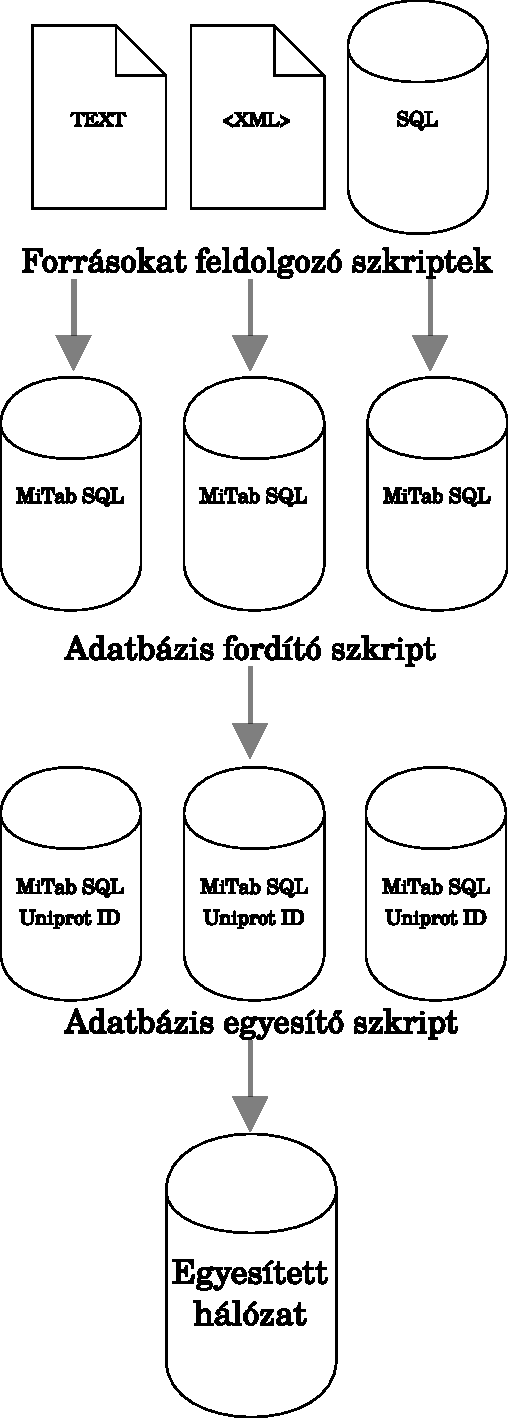
\includegraphics[scale=0.7]{img/Signalink_Layer0.pdf}
			 		 \centering

			 		 \caption{ \textbf{A hálózat létrehozásának folyamata} }
 
 			 		 \begin{imgdesc}
 				 		 A különböző forrásokból származó adatok esetén először a forrás formátumokat feldolgozni képes szkriptek átalakítják azokat a belső szabványként használt \textit{MiTab SQL} formátumra. Általában a különböző adatforrások különféle azonosítókkal illetik a komponenseiket. Ahhoz, hogy több hálózatot egyesíteni tudjunk, szükség van arra, hogy egy adott biológiai entitás csak egyfajta azonosítóval szerepeljen. A fordító szkript MiTab SQL fájlból olyan \textit{MiTab SQL} fájlt készít, amiben az elsődleges azonosító már a kivánt, esetemben \textit{Uniprot} azonosító. Legvégül az adatbázis egyesítő szkript úgy ``összefűzi" a különböző hálózatok pontjait és éleit, hogy ne legyen benne redundáns információ.
 			 		 \end{imgdesc}

			 		 \label{fig:slk3uml}			 		 
			 	 \end{figure}
			 	 



			
		 Az \textit{SQLite} adatbázisfájlok másik előnye, hogy rendelkezésünkre áll az \textit{SQL} nyelv. Mivel \textit{SQL} parancsok segítségével gyorsan kezelhetőek a feldolgozott adatok, így csak ritkán van szükség adatmanipulálási célból egy újabb szkript írására. Amennyiben mégis szükséges újabb szkript írása, a legtöbb szkriptnyelv rendelkezik valamilyen \textit{SQLite} adatbázis kezelési opcióval. Nagy méretű és mennyiségű biológiai adatot tároló \textit{SQLite} fájlban a keresés is igen gyorsan megoldható az adatbázis beindexelésével, sőt még gyorsabb keresés is megvalósítható az indexelt táblák memóriába csatolásával. Az \textit{SQLite} segítségével könnyen lehet importálni és exportálni a legtöbb népszerű adattárolási formátumba. Az előbb felsorolt okokból a csoportban a szöveges fájlok helyett az \textit{SQLite} adatbázisokat használjuk az adatok köztes tárolására. 
		
		Hálózatok tárolására a csoport által létrehozott \textit{MiTab SQL} formátumot használtam. A MiTab SQL egy \textit{SQLite 3}-ban tárolt a PSI-MI Tab formátummal közel megegyező adatstruktúra. A \textit{PSI-MI Tab} egy \textit{HUPO Proteomics Standards Initiative} (PSI) szervezet által meghatározott proteomikai adatok tárolására használt formátum. A PSI-MI Tab formátum specifikációja a szervezet honlapján elérhető. (\cite{hupo})
		
		A pontok és az élek külön táblában vannak letárolva az adatbázisban, így a \textit{PSI-MI Tab} specifikáció pontra és az élre vonatkozó tulajdonságai a megfelelő táblába kerülnek. A \textit{MiTab SQL} táblák oszlopai azonban nem teljesen egyeznek a \textit{PSI-MI Tab} kategóriákkal. Ilyen különbség például, hogy a \textit{MiTab SQL} nem használ néhány opcionális \textit{PSI-MI} kategóriát viszont tartalmaz a \textit{PSI-MI}-re nem jellemző tulajdonságokat is mint a topológia. Az éleket tartalmazó táblában a forrás (\textit{interactor\_a\_node\_name}) és a cél pont név oszlopa a \textit{node} tábla azonosító oszlopának idegen kulcsai. (\ref{fig:mitab_scheme}. ábra)
			
				\begin{figure}[H]
					 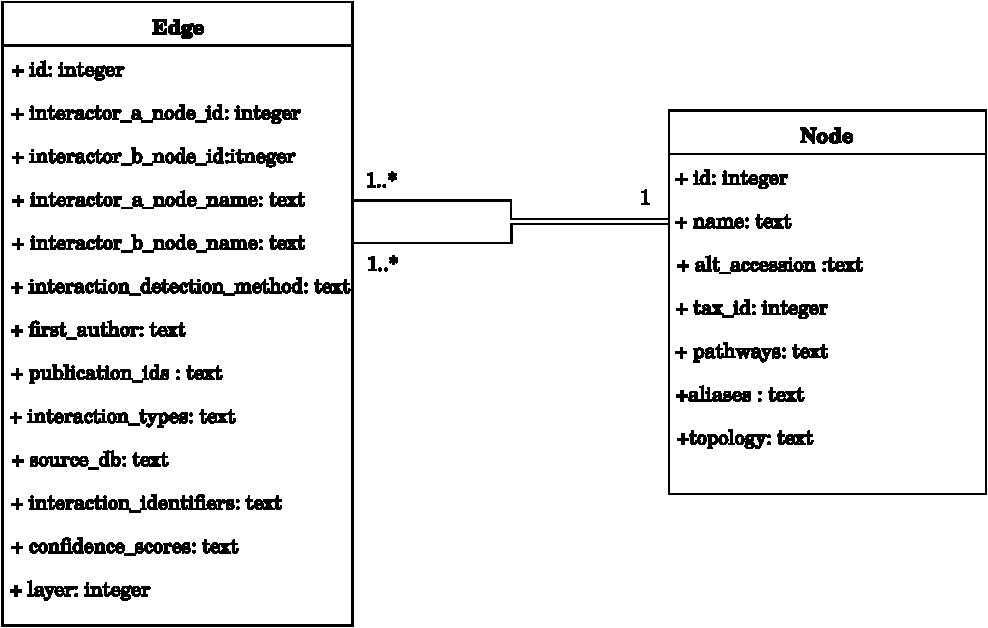
\includegraphics[scale=0.7]{img/Mitab-SQL.pdf}
			 		 \centering
			 		 \caption{ \textbf{A MiTab SQL sémája} }
			 		 \label{fig:mitab_scheme}			 		 
				\end{figure}
				
			\paragraph{Verziókövetés} \mbox{}\\
			Diplomamunkám készítése során a \textit{Git} verziókövető rendszert használtam, melynek tartalmát a web-alapú \textit{GitHub} tárhely szolgáltatásra töltöttem fel. A diplomamunkám \textit{GitHub} tárhelyén (\cite{github}) a következő általam írt kódok érhetők el: 
				\begin{itemize}
						\item A \ref{fig:slk3uml}. ábrán ábrázolt munkafolyamatot lebonyolító szkriptek
						\item A fordításhoz használt adatbázist megépítő szkript (Kadlecsik Tamás szkriptje alapján)
						\item A fordítást végző szkriptek
						\item Az adatbázisokat összeejtő szkriptek
						\item A MiTab SQL formátumot kezelő osztály
						\item A topológiai elemzést véző szkript
						\item Az adatszűrésre használt SQL szkriptek
				\end{itemize}
				
			\paragraph{Tesztelés} \mbox{}\\
			A bonyolultabb algoritmusok esetén \textit{egységteszteket (unit test)} alkalmaztam. A TI-t kiszámító \textit{Python} osztály összes metódusának működését ilyen módon ellenőriztem. A teszteléshez a \textit{pyhthon} saját \textit{unittest} nevű csomagját használtam.
				
			\paragraph{Adatok ábrázolása}
			A szakdolgozatomban látható képek és gráfok végleges formáját az \textit{InkScape} nevű ingyenes vektorgrafikus programmal állítottam elő. A gráfokat a \textit{Cytoscape} nevű hálózatelemző programmal készítettem.
			
\subsection{A források}
			
			\subsubsection{Autophagy Regulatory Network (\textit{ARN})}
			Az \textit{ARN} egy nagy terjedelmű autofágia adatbázis. Az adatbázis az irodalomból kézi gyűjtéssel kapott élek mellett tartalmaz még 19 más adatbázisból importált valamint 4 féle módszerrel prediktált kapcsolatokat is. Az \textit{ARN}-ben található 1485 darab fehérje között 4013 kapcsolat van. Az adatbázis komponensei között vannak az autofágia mechanizmusában szerepet játszó fehérjék és ezek regulátorai valamint transzkripciós faktorai. Az adatbázisban 413 transzkripciós faktor valamint 386 olyan miRNS melyek képesek lehetnek autofágia komponensek szabályzására(\cite{ARN}). \\
			Az ARN hat rétegből épül fel:
			\begin{enumerate}
				\item Autofágia fehérjék.
				\item Az első réteg fehérjéinek autofágia specifikus forrásokból származó regulátorai.
				\item Olyan poszt-transzlációs regulátorok melyek közvetlenül hatnak az első két réteg fehérjéire.
				\item Az első három réteg transzkripciós szabályzói.
				\item Az első négy réteg poszt-transzlációs regulátorai.
				\item Olyan jelátviteli útvonalak és fehérje-fehérje interakciók melyek különböző útvonalakat az autofágia szabályzóihoz kötnek (\cite{ARN}).
			\end{enumerate} 
					
			\subsubsection{Salmonet} 
			A \textit{Salmonet} a csoportunk által, jelenleg bírálat alatt álló molekuláris hálózat. A hálózat adatai kézi adatgyűjtésből, nagy áteresztőképességű módszerekből valamint predikciókból származnak. Az  integrált hálózat transzkripciónális szabályzási, metabolikus és fehérje-fehérje kölcsönhatási szinteket tartalmaz. A \textit{Salmonet} összesen öt-öt gasztrointesztinális és extraintesztinális \textit{Salmonella} törzs hálózatából lett egyesítve. Egy törzs hálózata a metabolikus, szabályzási és fehérje-fehérje alhálózatok egyesítéséből készült (\cite{salmonet}).
			
			A kapcsolatokat a nem fehérje-fehérje kölcsönhatási szinteken eltérően definiálhatók. Ha egy metabolit egy bizonyos reakció képződménye és egy másik szubsztrátja, akkor a két reakciót katalizáló fehérje kapcsoltnak tekinthető. Szabályzási kapcsolatnak pedig egy transzkripciós faktor a másik fehérje promóteréhez való kötődését értjük. 
			
			\subsubsection{Az ember-\textit{Salmonella} predikciók}
			Az eddig ismertetett források csak fajon belüli kapcsolatokból felépülő hálózatokat tartalmaztak. Ahhoz, hogy szakdolgozatomban tudjam tanulmányozni a humán-\textit{Salmonella} kapcsolatot szükségem van még interspecifikus élekre is. A predikciós forrásokból származó interspecifikus kapcsolatok fogják összekapcsolni a gazda hálózatát a patogénével. Szakdolgozatomban (\cite{Krishnadev}) és (\cite{Kshirsagar}) humán-\textit{Salmonella} predikcióit használtam.
			

		
		\subsection{Az források feldolgozásának eszközei}
		
			\paragraph{MiTab SQLite adatbázis API} \mbox{}\\
			A \textit{PsimiSQL} egy \textit{Python} 2.7-es szintaxisban írt osztály, melyet még a \textit{Signalink 3} összeállításához készítettem, de azóta más projektekben is használtam és továbbfejlesztettem. A \textit{PsimiSQL} segítségével a molekuláris biológiai hálózatok könnyen átalakíthatók \textit{MiTab SQLite} adatbázisokká. Az osztály számos függvényével megkönnyíti a \textit{MiTab SQLite} adatbázisok kezelését \textit{Python} alól. Ilyen függvény például a redundáns adatok adatbázisba illesztését gátló \textit{insert\_unique\_node()} mely ellenőrzi, hogy az adott hálózatban szerepel-e már az importálni kívánt pont. Az osztály példányosításakor a memóriában létrejön egy példányhoz kötött \textit{MiTab SQL} sémával rendelkező \textit{SQLite 3} adatbázis. Az adatbázis benépesítése és az adatok keresése tehát nagy sebességgel történik. Az osztálynak vannak olyan függvényei melyekkel könnyen importálni és exportálni lehet \textit{MiTab SQL} adatbázis fájlokat.
			
			\paragraph{A szótárak építése és a fordítás} \mbox{}\\
			Ahhoz hogy a feldolgozott forrásokat össze lehessen fűzni egy nagy adatszettbe, szükség van arra, hogy a hálózatokban ne szerepeljen ugyanaz a biológiai entitás más azonosítóval. Ennek érdekében mindegyik hálózat fehérjéit a legfrissebb \textit{Uniprot} adatbázis azonosítókra fordítottam amihez két szkriptet kellett írnom. 
			
			A \textit{Salmonet} és az \textit{ARN} már eleve \textit{Uniprot} azonosítókat használ. Azonban az \textit{Uniprot} adatbázis állandó frissítései miatt, fenn áll a lehetőség, hogy nem egy időben készült fájlok ugyanarra a fehérjére más \textit{Uniprot} azonosítót használnak. Egy másik hibaforrás az lehet, hogy a \textit{Uniprot} adatbázis egy fehérjét több azonosítóval is tárol. Amikor egy fehérjét beletesznek a \textit{Uniprot} adatbázisba, akkor kap egy elsődleges azonosítót. Primer azonosítót kapnak még olyan fehérjék is, melyek már benne voltak az adatbázisban de később külön izoformákra lettek szétválasztva. Új elsődleges azonosítót kapnak olyan fehérjék is melyeket több vélt fehérjéből egyesítettek. Minden ilyen művelet után, a legfrissebb elsődleges azonosító marad az új primer azonosító, az összes többi pedig másodlagos azonosítók lesznek. A \textit{Uniprot} azonosítókat még csoportosítani lehet az alapján is, hogy a fehérje manuálisan vagy automatikusan lett annotálva. Az első típusba az úgynevezett \textit{Swissprot} az utóbbiba pedig a \textit{trEMBL} azonosítók tartoznak. A szkriptem az összes pont azonosítójára, ha az nem \textit{Swissprot}, kikeresi a \textit{Swissprot} azonosítót ha létezik, vagy az elsődleges \textit{trEMBL} azonosítót. Az \textit{ARN} és a \textit{Salmonet} fordításához szükség volt egy \textit{Salmonella}-\textit{Salmonella} és egy humán-humán szótárra, amiket a Kadlecsik Tamás szótárépítő szkriptjével állítottam elő. Az azonosítókat a szótárak alapján saját készítésű szkripttel fordítottam.
			
			A predikciókhoz egy olyan szótárat kellett létrehozni, mely \textit{Salmonella} génazonosítókhoz rendel \textit{Salmonella} \textit{Uniprot} azonosítókat. Több okból is lehetséges ebben az esetben a génről fehérére fordítás. A \textit{Salmonella} adatbázisok általában csak génazonosítókat tartalmaznak, sőt vannak olyan publikált fehérje-fehérje kapcsolatokat leíró szövegfájlok is melyek csak génneveket tartalmaznak. Másik fő ok, az hogy \textit{Salmonell}ára még nincs megfelelő mennyiségű és felbontású adat. Valamint prokariótákban nincs alternatív splicing, így egy génről készülő fehérjék is jobban megfeleltethetőek. Ezt szintén Kadlecsik Tamás szkriptjével állítottam elő. Egy általam írt másik fordítószkript segítségével pedig az előzőhöz hasonló módon fordítottam a predikciókat.
			
			
	\subsection{A források feldolgozása}
			
		
	\paragraph{Az \textit{ARN} feldolgozása} \mbox{}\\
				A gazda patogén hálózat összeállításához az \textit{ARN} adatbázisnak csak az első, autofágia fehérjéket tartalmazó rétegét használtam fel. A hálózat letöltését követően azt egy általam írt \textit{Python} scripttel \textit{MiTab SQL} formátumba alakítottam. A fordító szkripttel az akkor legfrissebb \textit{Uniprot} adatbázis azonosítókra fordítottam. Mindezekre azért volt szükség, mert az \textit{ARN} létrehozásakor még nem használtuk a \textit{MiTab SQL} formátumot.	
				
	\paragraph{A \textit{Salmonet} feldolgozása} \mbox{}\\
				Az \textit{Salmonet} átalakítása az \textit{ARN}-hez hasonló módon történt, azzal a különbséggel, hogy fordításkor olyan szótárat használtam mely az összes \textit{Salmonella Uniprot} azonosítóhoz a legújabb \textit{Salmonella Uniprot} azonosítókat társítja.
				
	\paragraph{Az ember-\textit{Salmonella} predikciók feldolgozása}  \mbox{}\\
				A két predikció feldolgozására külön \textit{Python} szkripteket írtam. Csakúgy mint az előző forrásokat, az így elkészült adatbázisokat a legújabb \textit{Uniprot} azonosítóra fordítottam.
		

	\subsection{Az adatbázisok egyesítése}
		Az adatbázisok egyesítésekor a fő szempont az, hogy a végleges hálózatban ne legyenek redundáns pontok vagy élek. Az adatbázis egyesítő szkript beolvassa az összes adatbázisfájlt és egy \textit{has-map}ben eltárolja azok pontjait és éleit, valamint és ezek tulajdonságait. A \textit{hasm-map} adatstruktúra használatával sokkal gyorsabban kikereshető, hogy egy adott él vagy pont benne van-e a hálózatban, mint \textit{SQLite} adatbázisból. Amíg a szkript végigmegy az összes adatbázisfájlon a \textit{has-map}-ek tartalmából létrehoz egy \textit{MiTab SQL} fájlt mely már nem redundánsan tartalmazza az összes forrás adatbázis tartalmát.
		
		Az egyesített adatbázis tartalmazza a:
		\begin{itemize}
			\item A \textit{Salmonet} pontjait és fajon belüli kapcsolatait.
			\item Az \textit{ARN} pontjait és fajon belüli kapcsolatait.
			\item A predikciókból származó interspecifikus éleket
		\end{itemize}
		 
		 A predikciós élek közül is csak azokat tartottam meg, melynek mindkét nódusa megtalálható valamelyik kézi gyűjtésű forrásban. Tehát a predikciókból új pont nem került bele a hálózatba. Ezt az adatbázist már újabb \textit{Python} szkript írása nélkül csupán \textit{SQL} lekérdezésekkel hoztam létre.

	\subsection{A TopologyAnalyser osztály}
	
		A \textit{TopologyAnalyser} nevű osztályba csoportosítottam mindne olyan függvényt és változót mely a hálózatok topológiai elemzésével, a topológiai számítások elvégzésével, az éllisták feldolgozásával valamint az adatok importálásával és exportálásával foglalkozik. Ezáltal a hálózattal kapcsolatban álló összes függvény elérhető a TopologyAnalyser osztály metódusaként. A \textit{TopologyAnalyser} osztály \textit{Python 3} szintaxist használ. Az osztály segítségével többek közt kiszámítható a Jordán Ferenc féle TI$^n$. A \textit{TopologyAnalyser} egyetlen külső függősége a \textit{NetworkX} csomag. 
		
		A \textit{NetworkX} egy teljesen \textit{Python}ban írt, komplex hálózatok létrehozására, manipulálására és elemzésére használható ingyenes csomag. Vannak még más ingyenes hálózatkezelő \textit{Python} modulok, mint például a \textit{graph-tool} és az \textit{Igraph}. Az utóbbi kettő csomag már részben \textit{C/C++}-ban írták, így kisebb futásidőre képesek. Választásom mégis azért esett a kisebb teljesítményű \textit{NetworkX}-re mert így felhasználhattam régebben megírt szkriptjeimet.A \textit{Signalink} adatbázisának építésekor ugyanis szükségem volt például XGMML fájlok gyors feldolgozásársa, és erre a célra a \textit{NetworkX} egy alosztály használtam. 
		
		Az osztály konstruktorának egyetlen paramétere egy éllista. Példányosítás után a \textit{TopologyAnalyser} típusú objektum, egy éllistát, egy \textit{Graph} típusú objektumot és egy egység-élerősségi mátrixot tartalmaz.
		
		A \textit{Graph} osztály a \textit{NetworkX} csomag része és irányítatlan gráfok tárolására alkalmas. A hálózat példányhoz kötött \textit{Graph} típusú objektum (\textit{self.graph}) tárolása előnyös, mert így elérhetők a \textit{NetworkX} csomag különböző gráf elemzésre használható metódusai. Ilyen függvény például a \textit{Graph.neighbors\_iter(node)} mely egy adott pont szomszédjainak iterálható listáját adja vissza.
		
		Az élerősség mátrix (\textit{self.edgeStrength}) egy példányhoz kötött \textit{Python Dictionary}. A \textit{Dictionary} osztály   \textit{Pythonban} \textit{hashmap} adatstruktúrával van implementálva, ezáltal a benne tárolt adatok gyorsan elérhetők. A szótár kulcsai a mátrix indexei, az értékei pedig az élerősségek \textit{Fraction} típusú objektumokként letárolva. Az egységerő mátrix celláinak indexei maguk az élt alkotó pontok \textit{Uniprot} azonosítói. Az élerősség mátrix 0 értékkel rendelkező cellái nincsenek letárolva a \textit{hasmap}-ben.
		
		 A \textit{Fraction} objektumban a racionális számok két szám hányadosaként tárlódnak. Az törtszámok ilyen módú tárolása előnyös mert így elég csak akkor tizedestört formátumra hozni a számokat, ha már elvégeztük az összes műveletet. Ilyen módon sokkal pontosabb számításokat végezhetünk. Hátránya, az osztály a matematikából ismert tört műveleteket használja, így több számítást kell végezni.
		
		\paragraph{Az osztály fontosabb metódusai és működésük}

		\begin{itemize}
			\item \textit{getNthNeighbors()}
			
			A függvény rekurzívan kikeresi az adott pont $n$. szomszédját.
		
			\item \textit{pathFinder()}
			
			Ez a függvény megkeresi az összes $n$ hosszúságú útvonalat egy forrás és egy cél nódus között:
			
			  		\begin{algorithm}[H]
						\footnotesize
						
						\SetAlgoVlined
						\SetKwProg{Def}{def}{:}{}
						\Def{pathfinder(mélység, forrás nódus, cél nódus, útvonal, összegyűjtött útonalak)}{
							\uIf{útvonalhossz == 0}{
														forrás nódus hozzáadása az útvonalhoz \;
														mélység =- 1 
													}
													\uElseIf{mélység == 0 és forrás nódus == cél nódus}{
														\Return útvonal
													}
													\ElseIf{mélység == 0 és forrás nódus $\neq$ cél nódus}{
														\Return
													}
													
													\For{forrás nódus első szomszédai}{
														szomszéd nódus hozzáadása az útvonalhoz\;
														pathfinder( mélység - 1, szomszéd nódus, cél nódus, útvonal, összegyűjtött útvonalak) \;
														az utolsó pont eltávolítása az útvonalból\;
													}
						}
						
						
						
			  		\end{algorithm}
			  		
			  		\begin{imgdesc}
			  			A \textit{pathFinder metódus algoritmusának pszeudokódja}
			  		\end{imgdesc}
			  		
			\item \textit{buildEdgeUnitStrengthDict()}
			
			Ez a függvény egyszer hívódik meg a konstruktor lefutása során. A metódus imperatív módon egy \textbf{for} ciklussal végigiterál a kapott éllistán. A függvény visszatérési értéke egy egységerő mátrix.
			  		
			\item \textit{getNthPathwaysForNodes()}
			
			A függvény először minden pontnak megkeresi az $n$. szomszédját.  Mint az irodalmi bevezetőben ismertettem, a TI számolásánál páros lépésszámoknál az adott pont legalább egy hurkon keresztül eléri önmagát. A metódus két egymásba ágyazott \textbf{for} ciklust használ. A külső ciklus minden pontra előállítja a nódus $n$. szomszédjainak halmazát. A belső ciklus pedig minden cél és forrás pont párra meghívja a \textit{pathFinder()} függvényt, majd a kapott útvonalakat imperatívan hozzáadja egy listához, amit még a ciklusokon kívül definiáltam. A metódus visszatérési értéke egy lista amelyben minden lehetséges forrás és célpont közötti $n$ hosszúságú útvonal benne van.
			
			\item \textit{getEdgesFromPathway()}
			
			A metódus egy útvonalat fogad és az azt alkotó élek listájával tér vissza. 
			
			\item \textit{countPathwayStrength()}
			
			A metódus egy útvonalat kap, amire meghívja a \textit{getEdgesFromPathway} függvényt. Végigmegy a kapott éllistán és minden élre kikeresi a megfelelő értéket az egységerő mátrixból. Az összes él erejének összeszorzása után az út erősségével tér vissza.
			
			\item \textit{getPathWaysToNthNeighbours()}
			
			Ez a függvény kikeresi egy adott pont összes $n$. szomszédját és egy listában letárolja. Amikor elkészült a szomszédok listájával, akkor ezen egy \textbf{for} ciklus segítségével végigmegy. Ekkor minden periódusban meghívja a forrás és az aktuális cél nódusra a \textit{pathfinder} függvényt, majd a kapott útvonalakat imperatíven hozzáfűzi egy a cikluson kívül definiált listához. A ciklus után a függvény visszatér az elkészült listával.
			
			\item \textit{countTI()}
			
			A függvény egy adott pontra meghatározza annak TI értékét. Első lépésként létrehoz egy útvonal listát a \textit{getPathWaysToNthNeighbours} metódus segítségével, majd végigmegy az útvonalak listáján egy \textbf{for} ciklusban. Minden periódusban meghívja a \textit{countPathwayStrength(pathway)} függvényt az aktuális útvonalra, és annak eredményét egy a cikluson kívül definiált változóba akkumulálja.
			
		\end{itemize}
		\pagebreak


\section{Eredmények}

	Az elemzéseimet a \textit{Salmonet}, az \textit{ARN} és az egyesített hálózatra is elvégeztem. A TI-t mind a három hálóra kiszámoltam 1, 2 és 3 lépés távolságra. A TI alapján a három hálózat pontjaira rangsorokat írtam fel. Ezután megnéztem, hogy a különböző szempontokból fontosnak bizonyult fehérjék milyen biológiai funkciókat látnak el.
	
	\subsection{Topológiai indexek az alhálózatokban}
		\subsubsection{ARN}	
						
				Az \ref{table:arnti123}. táblázatban ábrázoltam az \textit{ARN}-re kiszámolt TI$^1$, TI$^2$ és TI$^3$  kategória első öt legfontosabb fehérjéit. A táblázatból látható, hogy egy adott fehérje különböző lépéshosszoknál számolt topológiai indexe nagyjából hasonló értékeket vesz fel. A TI$^2$ adatok mindenképp magukba foglalják azt, hogy a pontok hogyan hatnak vissza önmagukra. A TI$^3$-as értékek is tartalmazhatnak olyan útvonalakat melyeken egy pont önmagára visszahat, de csak akkor ha a két nódusnak van közös első szomszédja. A TI$^3$ tehát magába foglalja az adott pont önhatását de csak közvetett módon. A TI számításánál az egy pontba érő hatás ereje attól függ hogy a pontot hány darab útvonal éri el. Tehát TI számításánál az adott pontba érkező hatások összege mindig egy. Egy pont egységnyi erőt képes befogadni, ami a pontot elérő kapcsolatok között oszlik meg. A páros $n$ úthosszoknál az $n$. szomszédoktól érkező hatások mindenképp gyengébbek lesznek mert a pontra ható egység hatás még az önható útvonalak hatásával is megoszlik.
				
				\begin{table}[H]
				\centering
				\caption{Az \textit{ARN} legnagyobb TI értékű pontjai különböző lépésszámoknál}
				\label{table:arnti123}
				\begin{tabular}{|c!{\vrule width1.5pt}c|c!{\vrule width1.5pt}c|c!{\vrule width1.5pt}c|c|}
				\hline
				\textbf{Rang} & \textbf{Azonosító} & \textbf{TI$^1$} & \textbf{Azonosító} & \textbf{TI$^2$} & \textbf{Azonosító} & \textbf{TI$^3$} \\ \hline
				1.   & GABARAP            & 2,41                        & GABARAP            & 2,21                        & GABARAP            & 2,33                        \\ \hline
				2.   & MAP1LC3B           & 2,27                        & GABARAPL2          & 1,96                        & GABARAPL2          & 2,00                        \\ \hline
				3.   & BECN1              & 2,17                        & MAP1LC3C           & 1,93                        & MAP1LC3C           & 1,99                        \\ \hline
				4.   & MAP1LC3C           & 2,11                        & MAP1LC3B           & 1,75                        & MAP1LC3B           & 1,68                        \\ \hline
				5.   & ATG2A              & 1,99                        & ATG3               & 1,56                        & GABARAPL1          & 1,68                        \\ \hline
				\end{tabular}
				\end{table}
				
				
				\begin{figure}[H]
									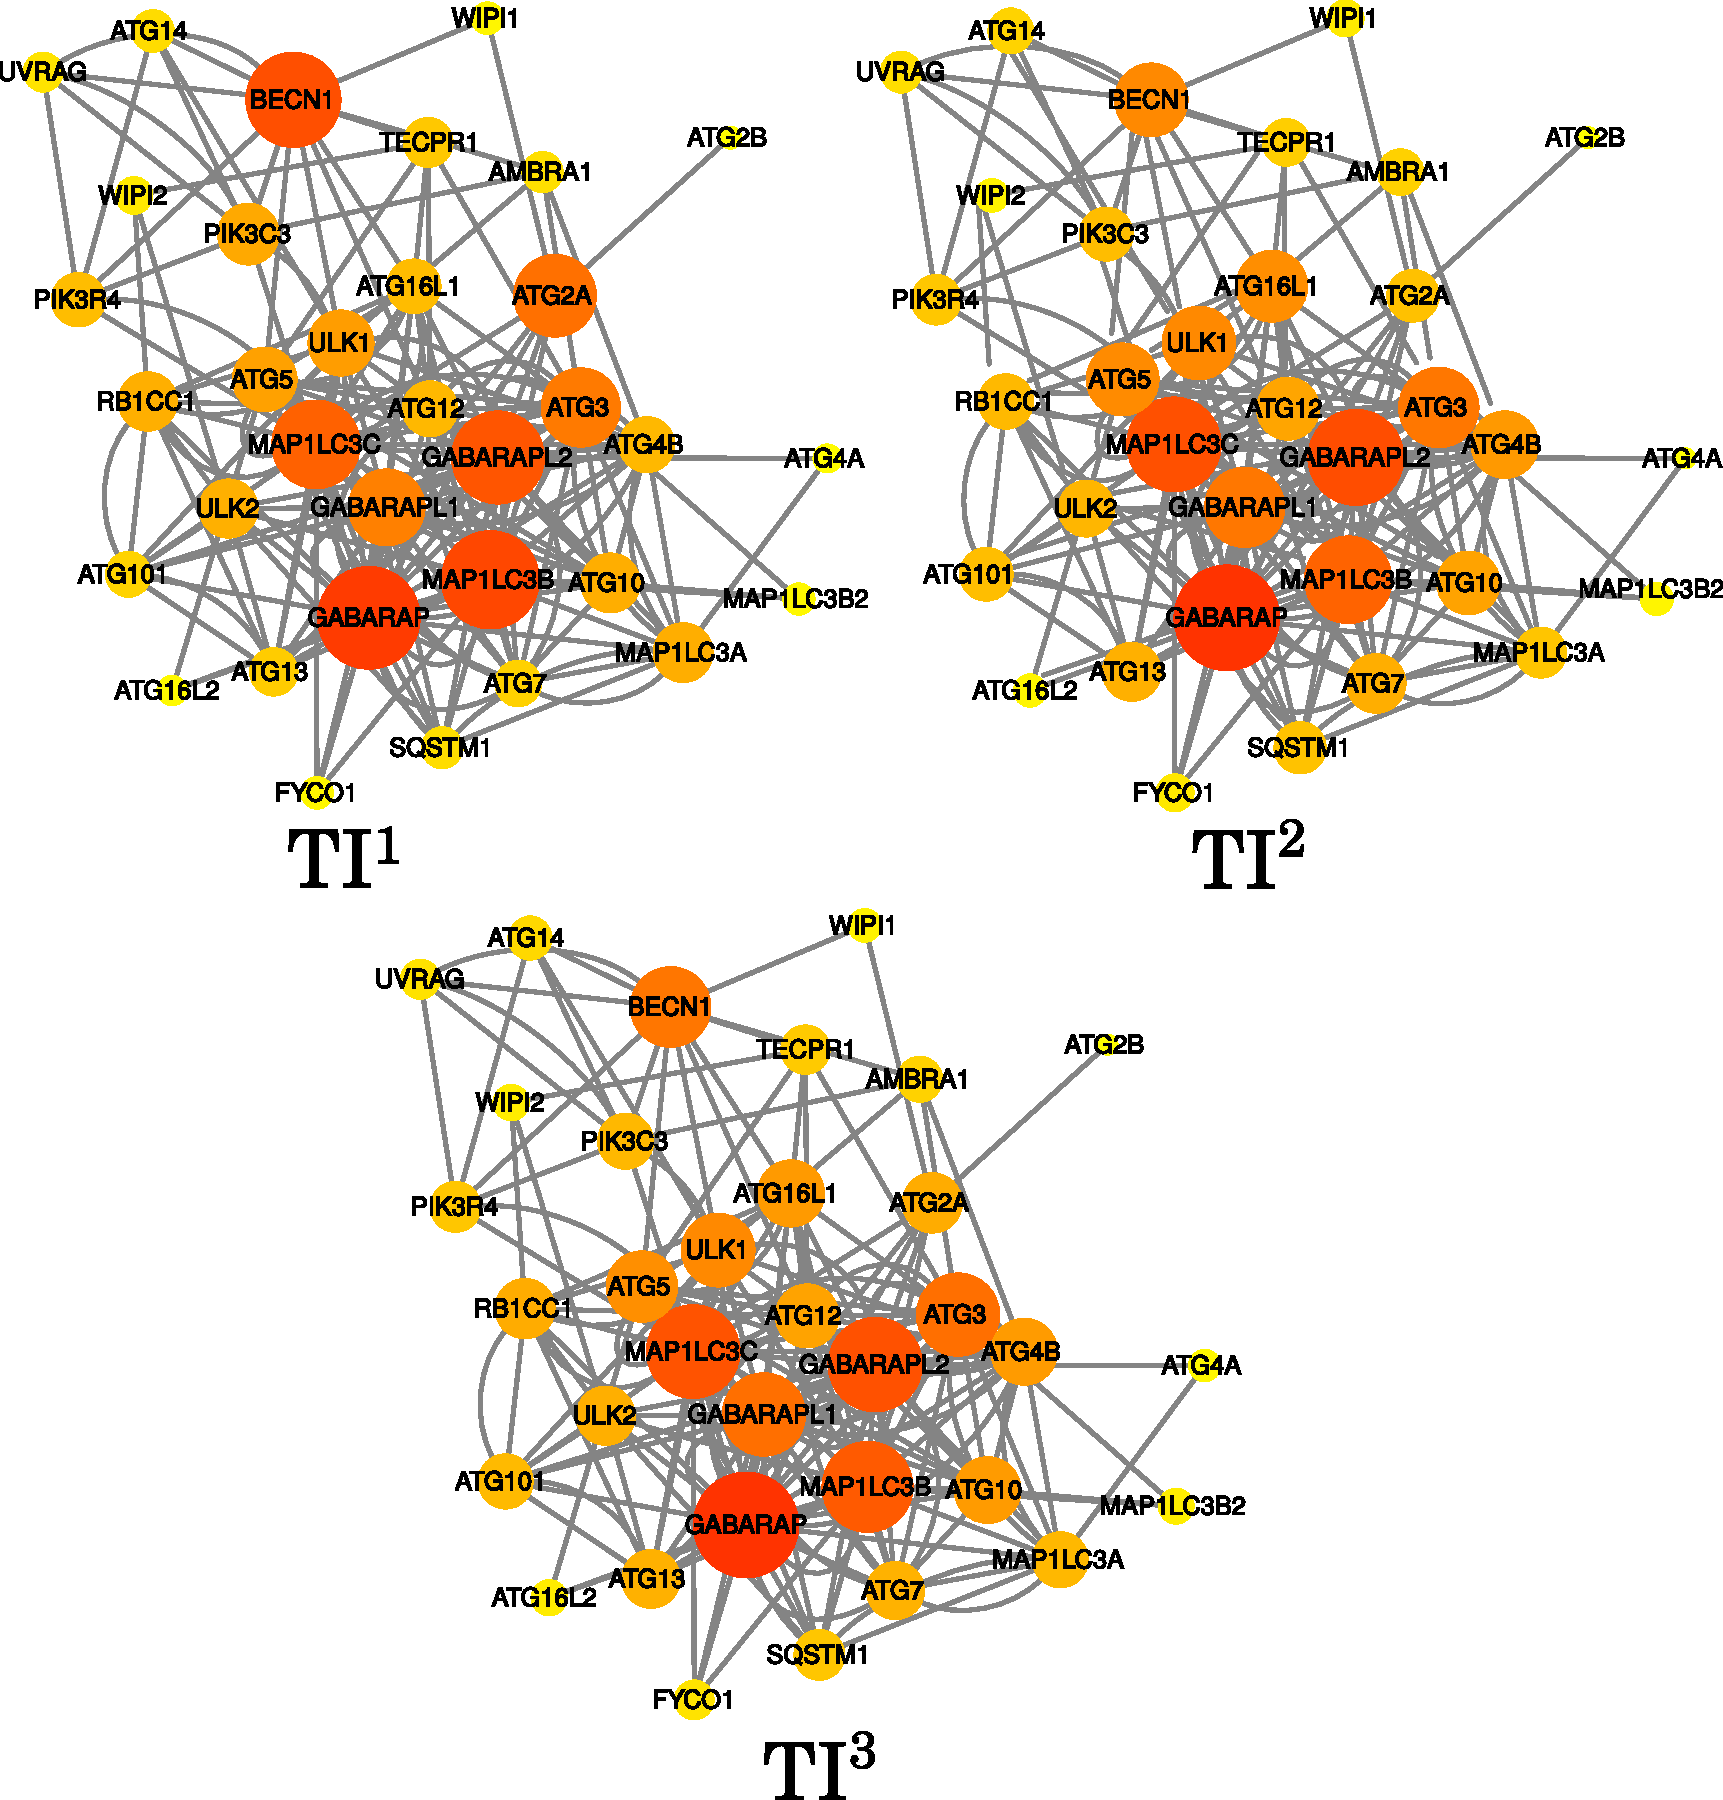
\includegraphics[scale=0.54]{img/arn_123_comp.pdf}
									\centering
									\caption{ \textbf{Az \textit{ARN} 1, 2 és 3 lépésre számított topológiai fontosságai}}
									\begin{imgdesc}
										A pontok színmélységét leíró skála a bal oldalon látható. Az ábra a különböző lépéshosszokra kiszámolt TI értékek eltéréseit szemlélteti. A többfajta lépéshosszra meghatározott indexek információt szolgáltatnak arról, hogy egy adott pont TI értéke hogyan változik egy hálózaton belül.
									\end{imgdesc}
						
									\label{fig:arn123}			 		 
				\end{figure}
				
				
				\paragraph{Az \textit{ARN} legnagyobb TI értékű fehérjéi} \mbox{}\\
				A következő felsorolásba összegyűjtöttem azokat a fehérjéket amelyek mind a három TI kategóriában megtalálhatók a tíz legfontosabb fehérje halmazában. 			
				A TI$^1$ a közvetlen topológiai hatást veszi legerősebben figyelembe. A három index közül a TI$^2$ fekteti a legnagyobb hangsúlyt az önhatásra. A TI$^3$  távolabbi szomszédságot is elérő közvetett hatás szempontjából fontos. A következő nyolc fehérje tehát mindegyik szempontból a benne van a legrangosabb pontok listáján:
				
				\begin{itemize}
					\item \textbf{ATG3} -- Más néven \textit{ubiquitine-like-conjugating enzyme ATG3}, egy konjugáló enzim, mely az autofágiában és a mitokondrium homeosztázisban tölt be szerepet. Autofágia során ez az enzim katalizálja a foszfatidiletanolamin konjugációját az ATG8 szerű fehérjék C-terminális glicinjére. Ilyen ATG8 szerű fehérje a listán szereplő GABRAP, GABARAPL1, GABARAPL2 valamint ezen a listán nem szereplő MAP1LC3A is \cite{autophagy_proteins}. 

					\item \textbf{BECN1} -- Más néven \textit{Beclin-1}. Az autofágia egyik kulcs fehérjéje. Bizonyos jelátviteli útvonalak hatására a VPS34-el együtt a fagofór kialakulását szabályozza. A \textit{Beclin-1} egy PI3K komplex alegysége, VPS34-el való kapcsolódása fokozza annak katalitikus hatását \cite{autophagy_proteins}. 
					
					\item \textbf{GABARAP, GABARAPL1 és a GABARAPL2} -- A GABARAP a nevét onnan kapta, hogy neuronokban a GABA$_A$ receptorokhoz kapcsolódik. A GABARAP egy 14kDa-os citoplazmatikus molekuláris \textit{chaperone}. Ma már tudjuk, hogy a fehérje ennél sokkal szélesebb körű kapcsolatrendszerrel rendelkezik. Autofágiában fagofór formálódásánál csakúgy mint az LC3-ak, a GABARAP-ok is liopidálódnak. Amikor egy sejtben az autofágia felpörög akkor a GABARAP-ek foszfatidiletanolaminra konjugált állapotban találhatóak, ezzel ellentétes helyzetben viszont konstitutív proteolítikus bomlásra vannak ítélve \cite{atg8_like}. 

					\item \textbf{MAP1LC3B} -- Ez a fehérje a MAP-ok családjába tartozik és emberben két majdnem identikus izoformája van. Első izoláláskor a MAP-1 alegységének vélték és ezért kapta LC3 (\textit{lighnt chain 3}) nevet. Az LC3 és a MAP1LC3B név tehát ugyanarra a fehérjére vonatkozik. Ma már tudjuk, hogy a mikrotubulusok mellett, az autofágiában is kulcsszerepet játszik \cite{atg8_like}.  Az autofágiában két ubikvitin rendszer szerű enzim-komplex dolgozik. Az LC3 autofágia indukciójakor proteolítikus hasítást szenved a citoplazmában és így jön létre az LC3B-I-es izoforma. Az LC3B-I-et az Atg7 egy E1-szerű enzim aktiválja, majd az E2 szerű ATG3-ra kerül. Ezután LC3B-I C-terminálisán helyezkedő glicinje foszfatidiletanolaminnal konjugálódik. Ez utóbbi formát nevezzük LC3B-II-nek. Az LC3B-II a növekvő fagofór külső és belső felszínén is megtalálható. Jelenlegi ismereteink alapján az LC3B-II két fő szerepei a membránok hemifúziója és a lebontásra irányított fehérjék szelekciója az autofagoszómához \cite{autophagy_proteins}. 
					
					\item \textbf{MAP1LC3C} -- Ez a fehérje egy LC3 paralóg, az \textit{LC3C} génről íródik át melynek szabályozása független az LC3-tól. Az LC3-hoz hasonlóan ez a fehérje is a makroautofágia szelektivitását növeli \cite{atg8_like}.
					
					\item \textbf{ULK1} -- Az ULK-1 egy szerin-threonin-protein-kináz, az ATG1 emlős homológja. Az ULK-1 a fagofór kéződés egyik kulcs faktora. Aktivitását az az mTORC1 szabályozza. Az mTORC1 egyik legfontosabb feladata emlős sejtekben az energiaszint érzékelés. Az mTORC1 magas tápanyagtartalom vagy aktiváló jelátvitel hatására foszforillálja az ULK-1 szubsztrátját, így az ULK-1 nem tudja beteljesíteni a fagofór kéződésében játszott szerepét és az autofágia gátlódik \cite{autophagy_proteins}. 
				\end{itemize}
				
		
		\subsubsection{Salmonet}
		
				A \textit{Salmonet} 2425 nódust és 7973 élt tartalmaz. A \textit{Salmonet} jobban hasonlít az egyesített hálózatra. Az \textit{ARN}-el ellentétben de az integrált hálózathoz hasonlóan, jóval  magasabbak a legnagyobb TI-vel rendelkező pontjainak értékei. Sőt a \textit{Salmonet} különböző lépésszámokhoz rendelt öt legfontosabb fehérjéinek listája megegyezik az egyesített hálózatéval (\textit{\ref{table:salmonet123}. és \ref{table:merged123}. táblázat}). 
										
				\begin{table}[H]
				\centering
				\caption{A \textit{Salmonet} legnagyobb TI értékű pontjai különböző lépésszámoknál}
				\label{table:salmonet123}
				\begin{tabular}{|c!{\vrule width1.5pt}c|c!{\vrule width1.5pt}c|c!{\vrule width1.5pt}c|c|}
				\hline
				\textbf{Rang} & \textbf{Azonosító} & \textbf{TI$^1$} & \textbf{Azonosító} & \textbf{TI$^2$} & \textbf{Azonosító} & \textbf{TI$^3$} \\ \hline
				1.   & phoP               & 64,46                       & trxA               & 16,61                       & phoP               & 53,84                       \\ \hline
				2.   & ssrB               & 59,77                       & phoP               & 10.30                       & ssrB               & 49.06                       \\ \hline
				3.   & rpoN               & 46,89                       & yajL               & 9.95                        & rpoN               & 38.11                       \\ \hline
				4.   & hilD               & 39,87                       & hilD               & 8,70                        & hilD               & 31,20                       \\ \hline
				5.   & trxA               & 23,77                       & ssrB               & 7,70                        & trxA               & 20.11                       \\ \hline
				\end{tabular}
				\end{table}
				
				A \textit{Salmonet} már túl sok pontot és kapcsolatot tartalmaz, hogy a különböző TI értékeit a \textit{\ref{fig:arn123}}. ábrához hasonlóan látványosan lehessen szemléltetni. A TI jellemzésére viszont ilyen nagy hálózatokra is kiváló lehetőséget nyújtanak az ökológiában használt rang abundancia diagramok. A \textit{Salmonet} rang abundancia diagramjainak lefutásai, hasonló mintázatot adnak, mint a Jordán és munkatársai által ökológiai hálózatok TI értékeire felírható görbék (\cite{ti}).
				
				\begin{figure}[H]
						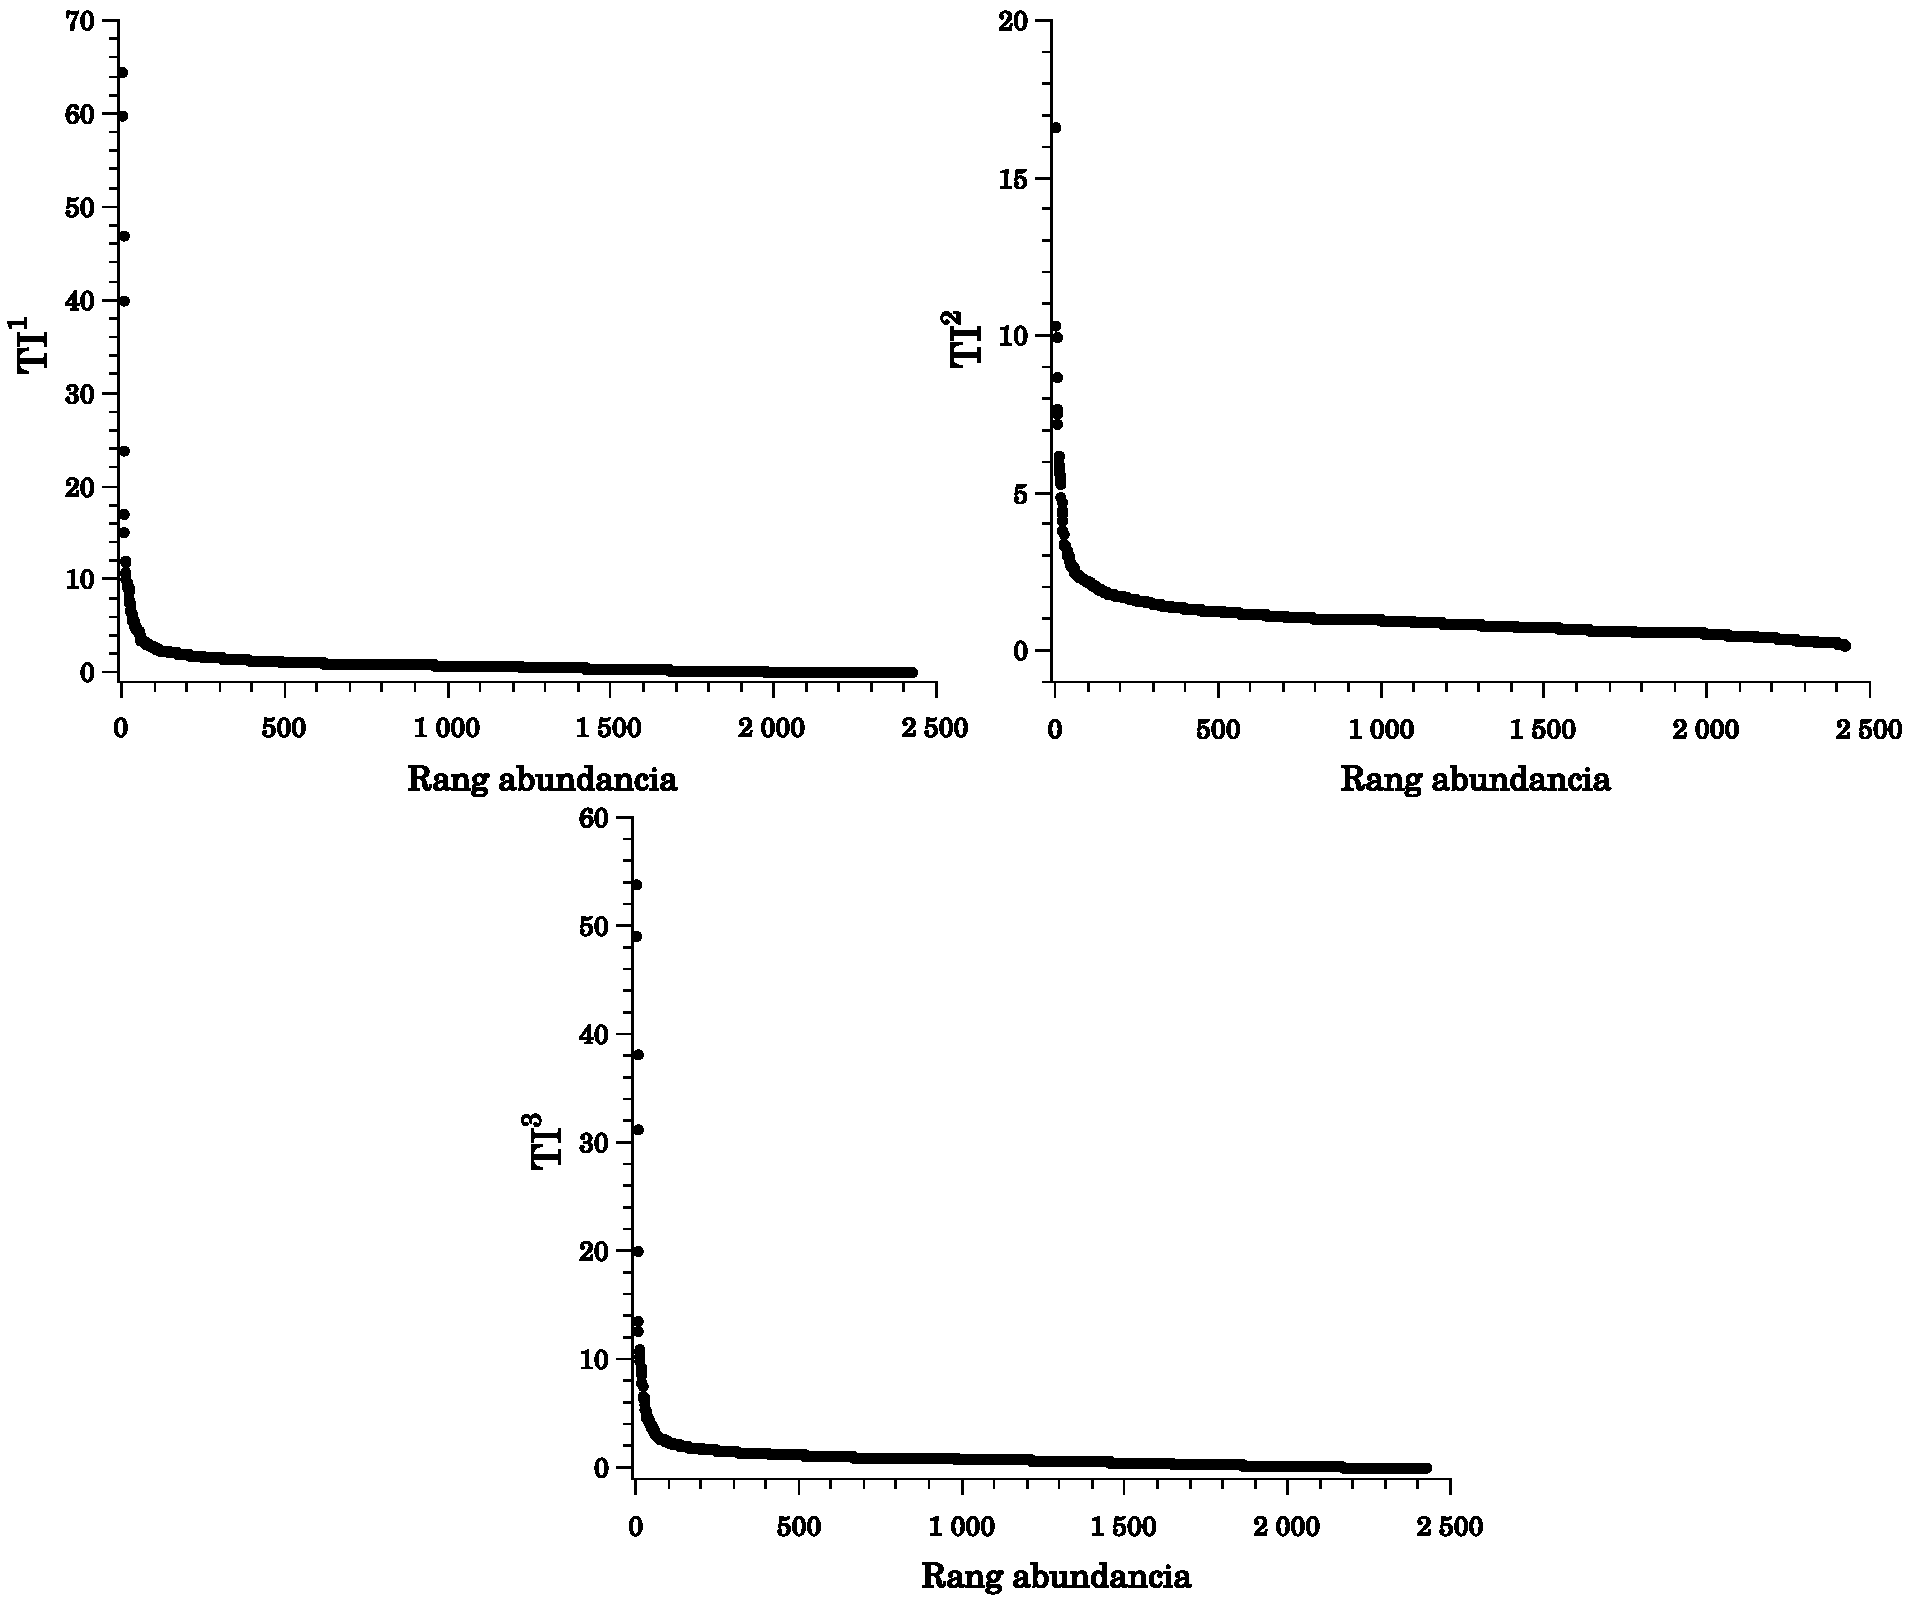
\includegraphics[scale=0.44]{img/salmonet_tis.pdf}
						\centering
						\caption{ \textbf{A \textit{Salmonet} pontjainak rang abundancia diagramjai}}
						\begin{imgdesc}
							Az ábrán látható grafikonokon a \textit{Salmonet} pontjai a különböző TI értékek szerint sorba vannak rendezve. 
						\end{imgdesc}
			
						\label{fig:salmonet_stats}			 		 
				\end{figure}
				
			A \textit{Salmonet}-ben négy olyan fehérje van mely mind a három topológiai index szempontjából a legerősebb tíz helyezettben van:
			
			\begin{itemize}
				\item \textbf{hilD} -- \textit{Salmonella} Typhimuriumban a patogenitási sziget 1 (SPI-1) kódolja a T3SS fehérjéit amik az invázióhoz szükségesek. Az SPI-1 génjei többnyire a szigeten kívüli transzkripciós faktorok által szabályozódnak. A sziget mester transzkripciós faktora a hilA, melyet két másik fehérje mellett a hilD szabályoz. A hilD-nek eddig 17 kötési helyét írták le a \textit{Salmonella} genomban (\cite{hilD}). 

				\item \textbf{phoP} -- A T3SS komponenseit kódoló patogenitási sziget mellett egy másik fontos virulencia rendszer is szerepet játszik a \textit{Salmonella} fertőzés sikerességében. 
				A phoP-phoQ egy kétkomponensű rendszer mely intracelluláris szignálokra aktiválódik, és nélkülözhetetlen a baktériumsejtek túléléséhez és replikációjához. A phoQ egy kináz mely a megfelelő jelátvitel hatására foszforilállja a phoP-t ami ekkor ki tudja fejezni transzkripciós aktivátor hatását (\cite{phoP}). 
				
				\item \textbf{ssrB} -- Az ssrA-ssrB is egy kétkomponensű rendszer mely szintén egy szenzor kinázból és egy regulátor transzkripciós faktorból áll. Az ssrA-ssrB rendszer szükséges a baktériumsejtek makrofágokon belüli túléléséhez és replikációjához. A PSI-2 (patogenitási sziget 2) több ssrB promótert is tartalmaz. Az ssrB több gén mellett az SPI-2-ben kódolt T3SS fehérjéinek átírásáért is felelős (\cite{ssrB}). 
				
				\item \textbf{trxA} -- A trxA is egy több komponensű rendszer része. A trxA egyike a \textit{Salmonella} genom két ismert thioredoxinjának. A trxA által kódolt fehérje a trx1 egy kicsi oldható diszulfid reduktáz enzim.  A trx1 sok specifikus célfehérjéinn thiol-diszulfid redox folyamatot hajt végre, így fontos szerepet játszik az oxidatív stressz elleni védelemben. Az oxidált trx1 a redukált trxB-ből regenerálódik, mely NADPH-ból szerzi a redukálóerőt (\cite{trxA}). 
			\end{itemize}
			
	\subsection{Topológiai indexek az integrált hálózatban}
	
		Eddig csak adott hálózaton belül hasonlítottam össze a pontok topolügiai fontosságát. Azonban fontos információt nyújt az is, hogy egy pont TI értéke hogyan változik azzal, hogy az eredeti vagy az egyesített hálózatban vizsgáljuk.
	
		Az egyesített hálózat az \textit{ARN}-nél jóval kompaktabb, az \textit{ARN}-ben pontok a kevésbé gazdagon kapcsoltak egymással. Az egyesített hálózat denzitása 0,00136 \%, míg az \textit{ARN}-é 0,00099\%. A denzitási értékekkel ellentétesen az \textit{ARN}-ben nagyobb az olyan nódusok aránya melyeknek nagy a TI értéke. Az egyesített hálózatban csupán a pontok 31,9\%-a rendelkezett egynél nagyobb TI$^3$ értékkel, ugyanakkor ez az arány az \textit{ARN} esetén már 44,1\%.
		
		A feldolgozott \textit{ARN} hálózat 34 pontot tartalmaz amik között 186 él van. A \textit{Salmonet}-ben pedig 2425 pont van amik között 7973 él húzódik. A predikciók az \textit{ARN}-ből és \textit{Salmonet}-ből származó 2459 nódus közé még 40 kapcsolatot adnak. A végleges hálózat így 2459 pontot és 8199 élt tartalmaz.
			
					\begin{figure}[H]
						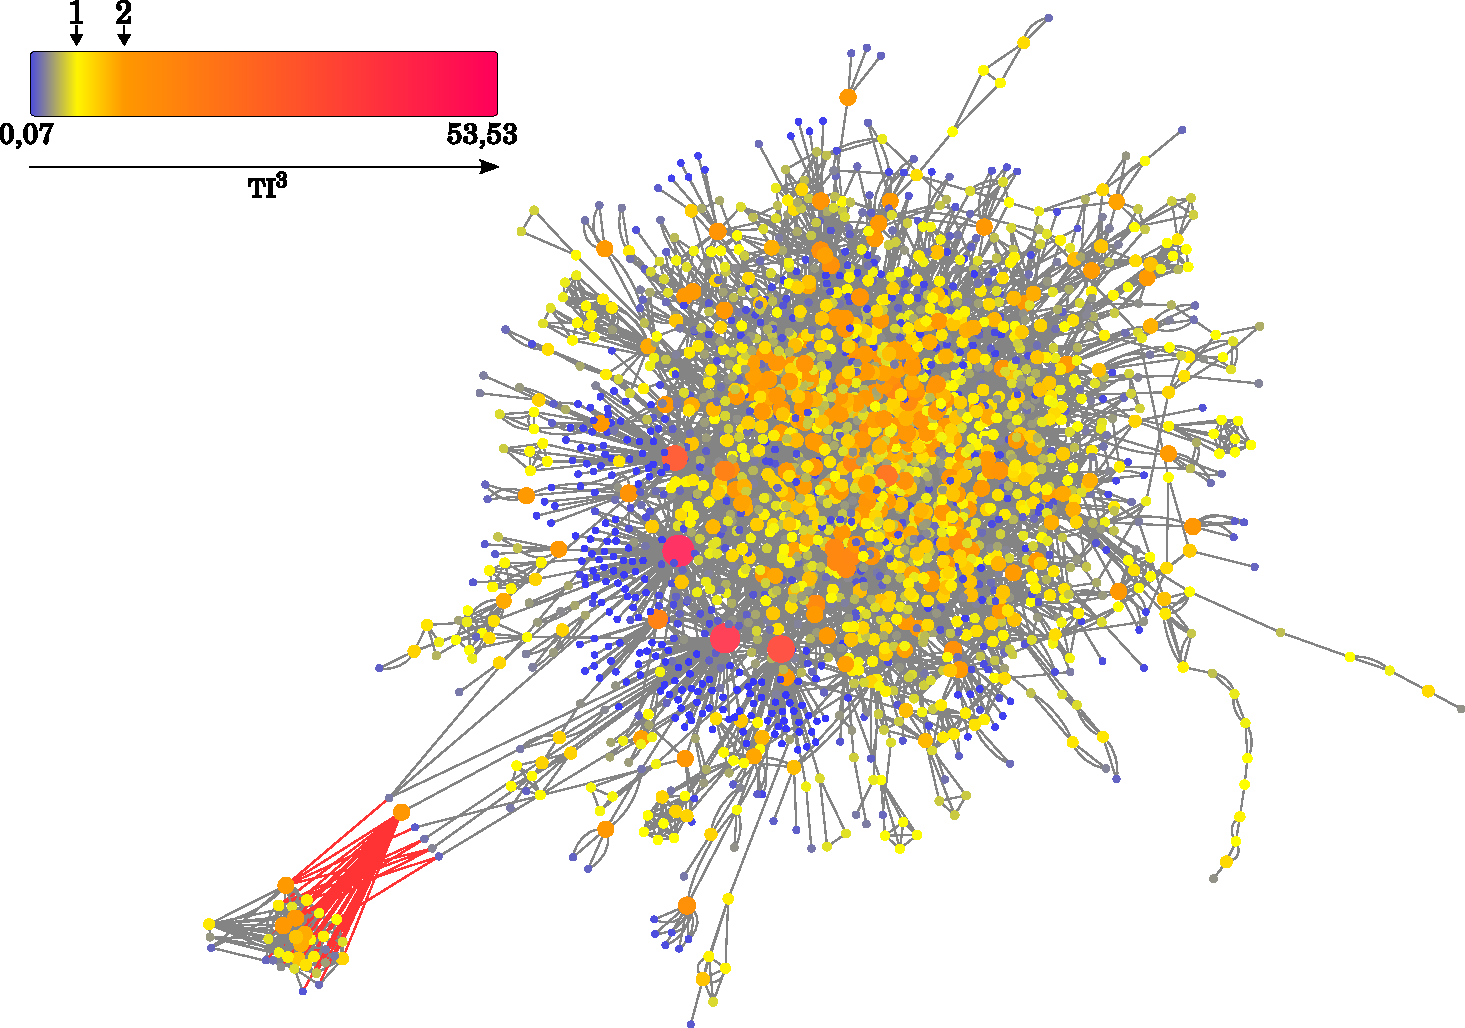
\includegraphics[scale=0.6]{img/merged.pdf}
						\centering
						\caption{\textbf{ Az egyesített hálózat}}
						\begin{imgdesc}
							A hálózaton piros élek jelölik az \textit{ARN}-t (\textit{baloldalt alul}) és a \textit{Salmonet}-et elválasztó prediktált éleket. Az ábrán a színátmenetek és méretek arányosak a pontokra kiszámolt TI$^3$-al. A színátmenetet szemléltető nem lineáris skála a bal felső sarokban látható. A topológiailag fontos pontok kiemelése érdekében három csoportot állítottam fel: Az első csoportba azok a pontok tartoznak, melyekből távozó hatás kisebb vagy egyenlő mint a beérkező (TI$^3\leq1$). A hálózatban 1674 ilyen nódus található, ami a hálózat 68,1\%-át teszi ki. Az utóbbi pontok színe a sötétkéktől a citromsárgáig terjed. A középső a színskálán citromsárgától narancsig terjedő kitöltésű pontok azok melyeknek már van nettó kimenő hatásuk ($1<$TI$^3<2$). Ebbe a halmazba 624 pont azaz a hálózat 25,4\%-a tartozik. A harmadik narancstól vörösig terjedő csoportot azok a nódusok alkotják melyeknek a legnagyobb a TI értékük. Ez utóbbi 161 pont a hálózat 6,5\%-át teszi ki.
						\end{imgdesc}
			
						\label{fig:merged}			 		 
					\end{figure}		
					
					\begin{table}[H]
					\centering
					
					\caption{
						\textbf{Az egyesített hálózat legnagyobb TI értékkel rendelkező pontjai különböző lépésszámoknál}
					}
					\label{table:merged123}


					\begin{tabular}{|c!{\vrule width1.5pt}c|c!{\vrule width1.5pt}c|c!{\vrule width1.5pt}c|c|}
					\hline
					\textbf{Rang} & \textbf{Azonosító} & \textbf{TI$^1$} & \textbf{Azonosító} & \textbf{TI$^2$} & \textbf{Azonosító} & \textbf{TI$^3$} \\ \hline
					1.      & phoP               & 64,38                       & trxA               & 16,61                       & phoP               & 53,53                       \\ \hline
					2.      & ssrB               & 59,17                       & phoP               & 10.31                       & ssrB               & 46,15                       \\ \hline
					3.      & rpoN               & 46,21                       & yajL               & 9.95                        & rpoN               & 37.36                       \\ \hline
					4.      & hilD               & 39,79                       & hilD               & 8,71                        & hilD               & 31,07                       \\ \hline
					5.      & trxA               & 23,77                       & ssrB               & 7,93                        & trxA               & 20.10                       \\ \hline
					\end{tabular}

					\end{table}	 			
						
			Az integrált hálózatban a \textit{Salmonet} tulajdonságai érvényesülnek. Az első öt nódus mind a három TI kategóriájában \textit{Salmonet} eredetű. (\textit{\ref{table:merged123}. táblázat})  A hálózatban a legerősebb hatással rendelkező humán fehérje a GABARAP, ami TI$^1$ (2,54) és TI$^3$ (2,12) esetén a 88., TI$^2$-nél (2,61) pedig a 112. legerősebb hatású pontnak számít.   
			
			A hálózat fontossági rangsorára felrajzolhatók az ökológiában alkalmazott rang abundancia diagramok.  (\textit{\ref{fig:mergedTIs}. ábra}) A rang abundancia diagramok \textit{x} értékei a pontok rangsorszámai. Az értékkészletük pedig a pontra vonatkoztatott valamilyen mérőszám értékeinek halmaza. Ebben az esetben az \textit{y} értékek a különböző lépéshosszhoz számított TI-k.
			
			A \textit{\ref{fig:mergedTIs}. ábrán} megfigyelhető, hogy a hálózatban csupán néhány kiugróan magas TI értékű pont van. Az is jól látszik, hogy a visszahatást figyelmen kívül hagyó TI$^1$ és a csak közvetett útvonalakon közvetített önhatást figyelő TI$^3$ közel azonos lefutású. TI$^2$-nél minden pont eléri önmagát az összes első szomszédján keresztül. Egy pont hatása a cél pontja fokszámával fordítottan arányos. A megnövekedett bemenetszámok miatt a TI$^2$ értékek is kisebbek, viszont jól szemléltetik azt, hogy az adott pontok mennyire hatnak vissza önmagukra			
			
			\begin{figure}[H]
				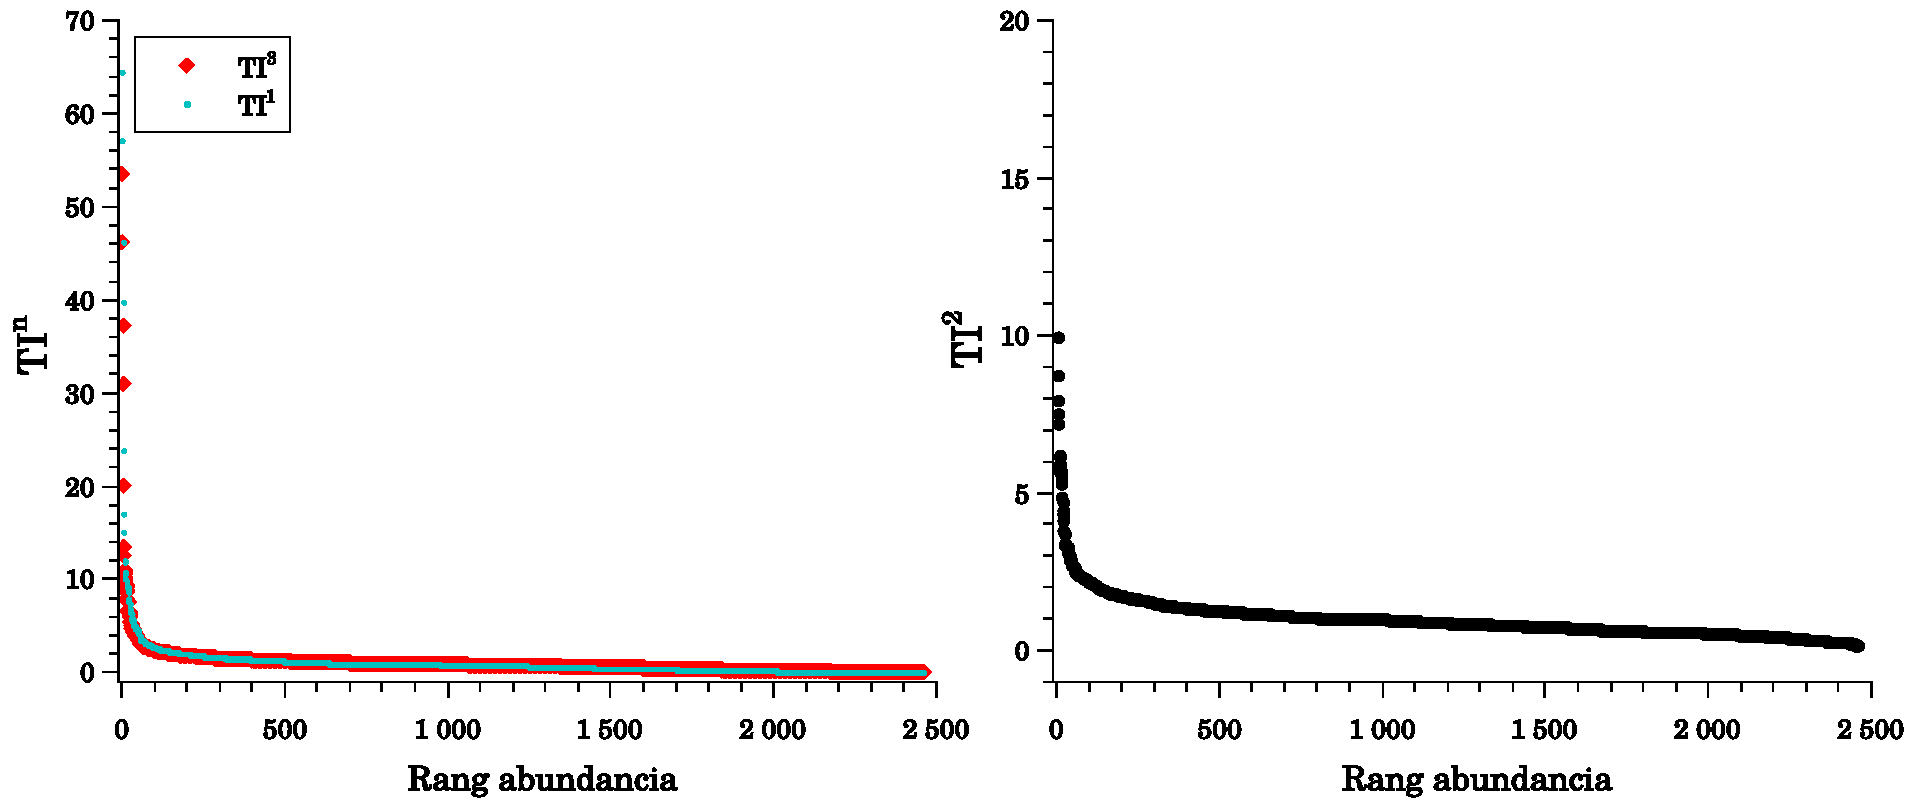
\includegraphics[scale=0.5]{img/mergedTIs.pdf}
				\centering
				\caption{\textbf{ Az egyesített hálózat rang abundancia görbéi}}
				\begin{imgdesc}
					Az ábra bal oldalán a TI$^1$ pontjai pirossal, a TI$^3$ pedig kékkel. Jól látható, hogy a TI$^1$ és a TI$^3$ lefutása nagyjából azonos. A jobb oldalon a TI$^2$ pontjai láthatóak. A két grafikon skálázása alapján leolvasható, hogy a TI$^2$ értékei kisebbek a TI$^1$ és TI$^3$ értékeitől.
				\end{imgdesc}
	
				\label{fig:mergedTIs}			 		 
			\end{figure}


			\begin{figure}[H]
				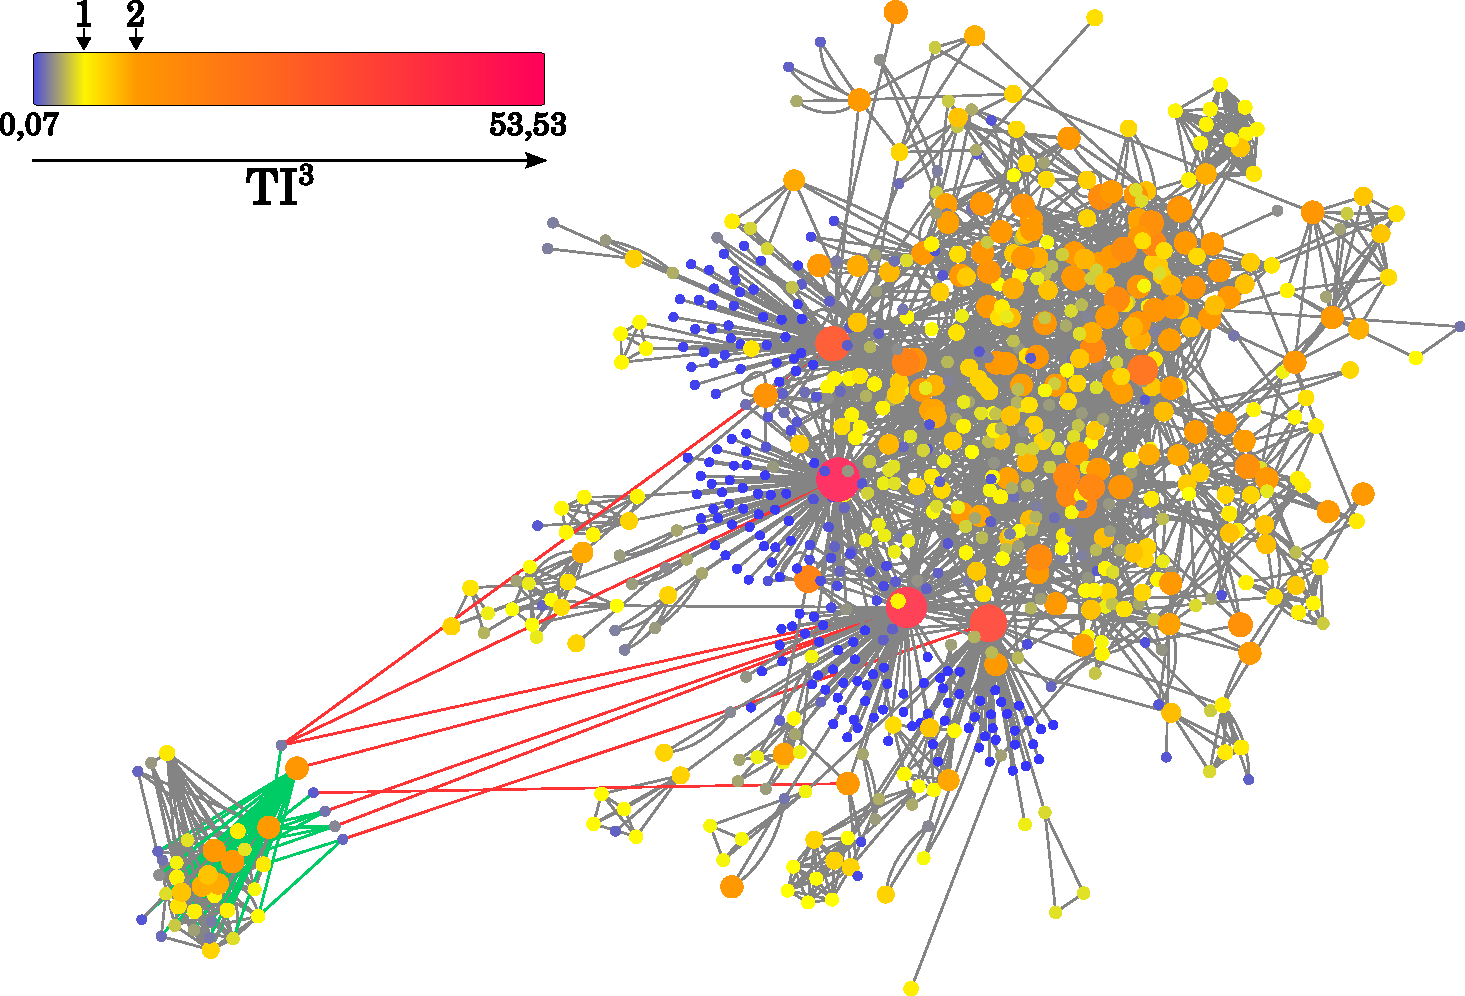
\includegraphics[scale=0.50]{img/merged-3-step-from-connecting-salmonella.pdf}
				\centering
				\caption{ \textbf{Az interfész fehérjéktől három lépésre elérhető pontok}}
				\begin{imgdesc}
					Az ábra az egyesített hálózat azon részét tartalmazza mely elérhető három lépésre a \textit{Salmonella} hat darab interfész fehérjéjétől. Ez az a környezet, ahol az interfészfehérjék TI$^3$-at alkotó topológiai hatásai érvényesülnek. A zöld színű élek a predikciókból származnak és a \textit{Salmonetet} \textit{(jobb)} kötik össze az \textit{ARN}-el \textit{(bal)}. A piros színű élek ez esetben a \textit{Salmonella} interfész fehérjéi és ezek \textit{Salmonellán} belüli első szomszédai között húzódnak. Látványos, hogy ez utóbbi élekből a legtöbb a legerősebb TI értékű pontokhoz tart. A pontok színezése megegyezik az \ref{fig:merged}. ábránál ismertetett sémával, a színskála a bal felső sarokban látható.
				\end{imgdesc}			
				\label{fig:merged-3-step}			 		 
			\end{figure}			
		
	\subsection{A hármas típusú szekréciós rendszer kapcsolatai}	
		
		\subsubsection{A \textit{Salmonella} kapcsolatai az autofágia fehérjékkel}
		
		Az \textit{ARN} fehérjéiből 30 létesít összesen 40 kapcsolatot valamilyen \textit{Salmonella} fehérjével. A predikciók alapján tehát hálózatban szereplő humán autofágia fehérjék 88\%-a létesíthet kapcsolatot \textit{Salmonella} fehérjével \textit{(\ref{fig:connection}. ábra)}.
		
		 A 40 darab fajok közötti kapcsolatért \textit{Salmonella} oldalról csupán a következő hat \textit{Salmonella} fehérje a felelős: sifB, slpA, sopB, sseI, sseL, sspH2 (\textit{\ref{fig:connection}. ábra}). A predikciók alapján tehát a \textit{Salmonella} fehérjék mindössze 0,2\%-a létesít csak kapcsolatot a gazda autofágia fehérjéivel. Az ábrán az is megfigyelhető, hogy a négy csak humán kapcsolattal rendelkező fehérje viszonylag kisebb TI-vel rendelkezik, pedig valóban központi szerepűek.
		
				\begin{figure}[H]
					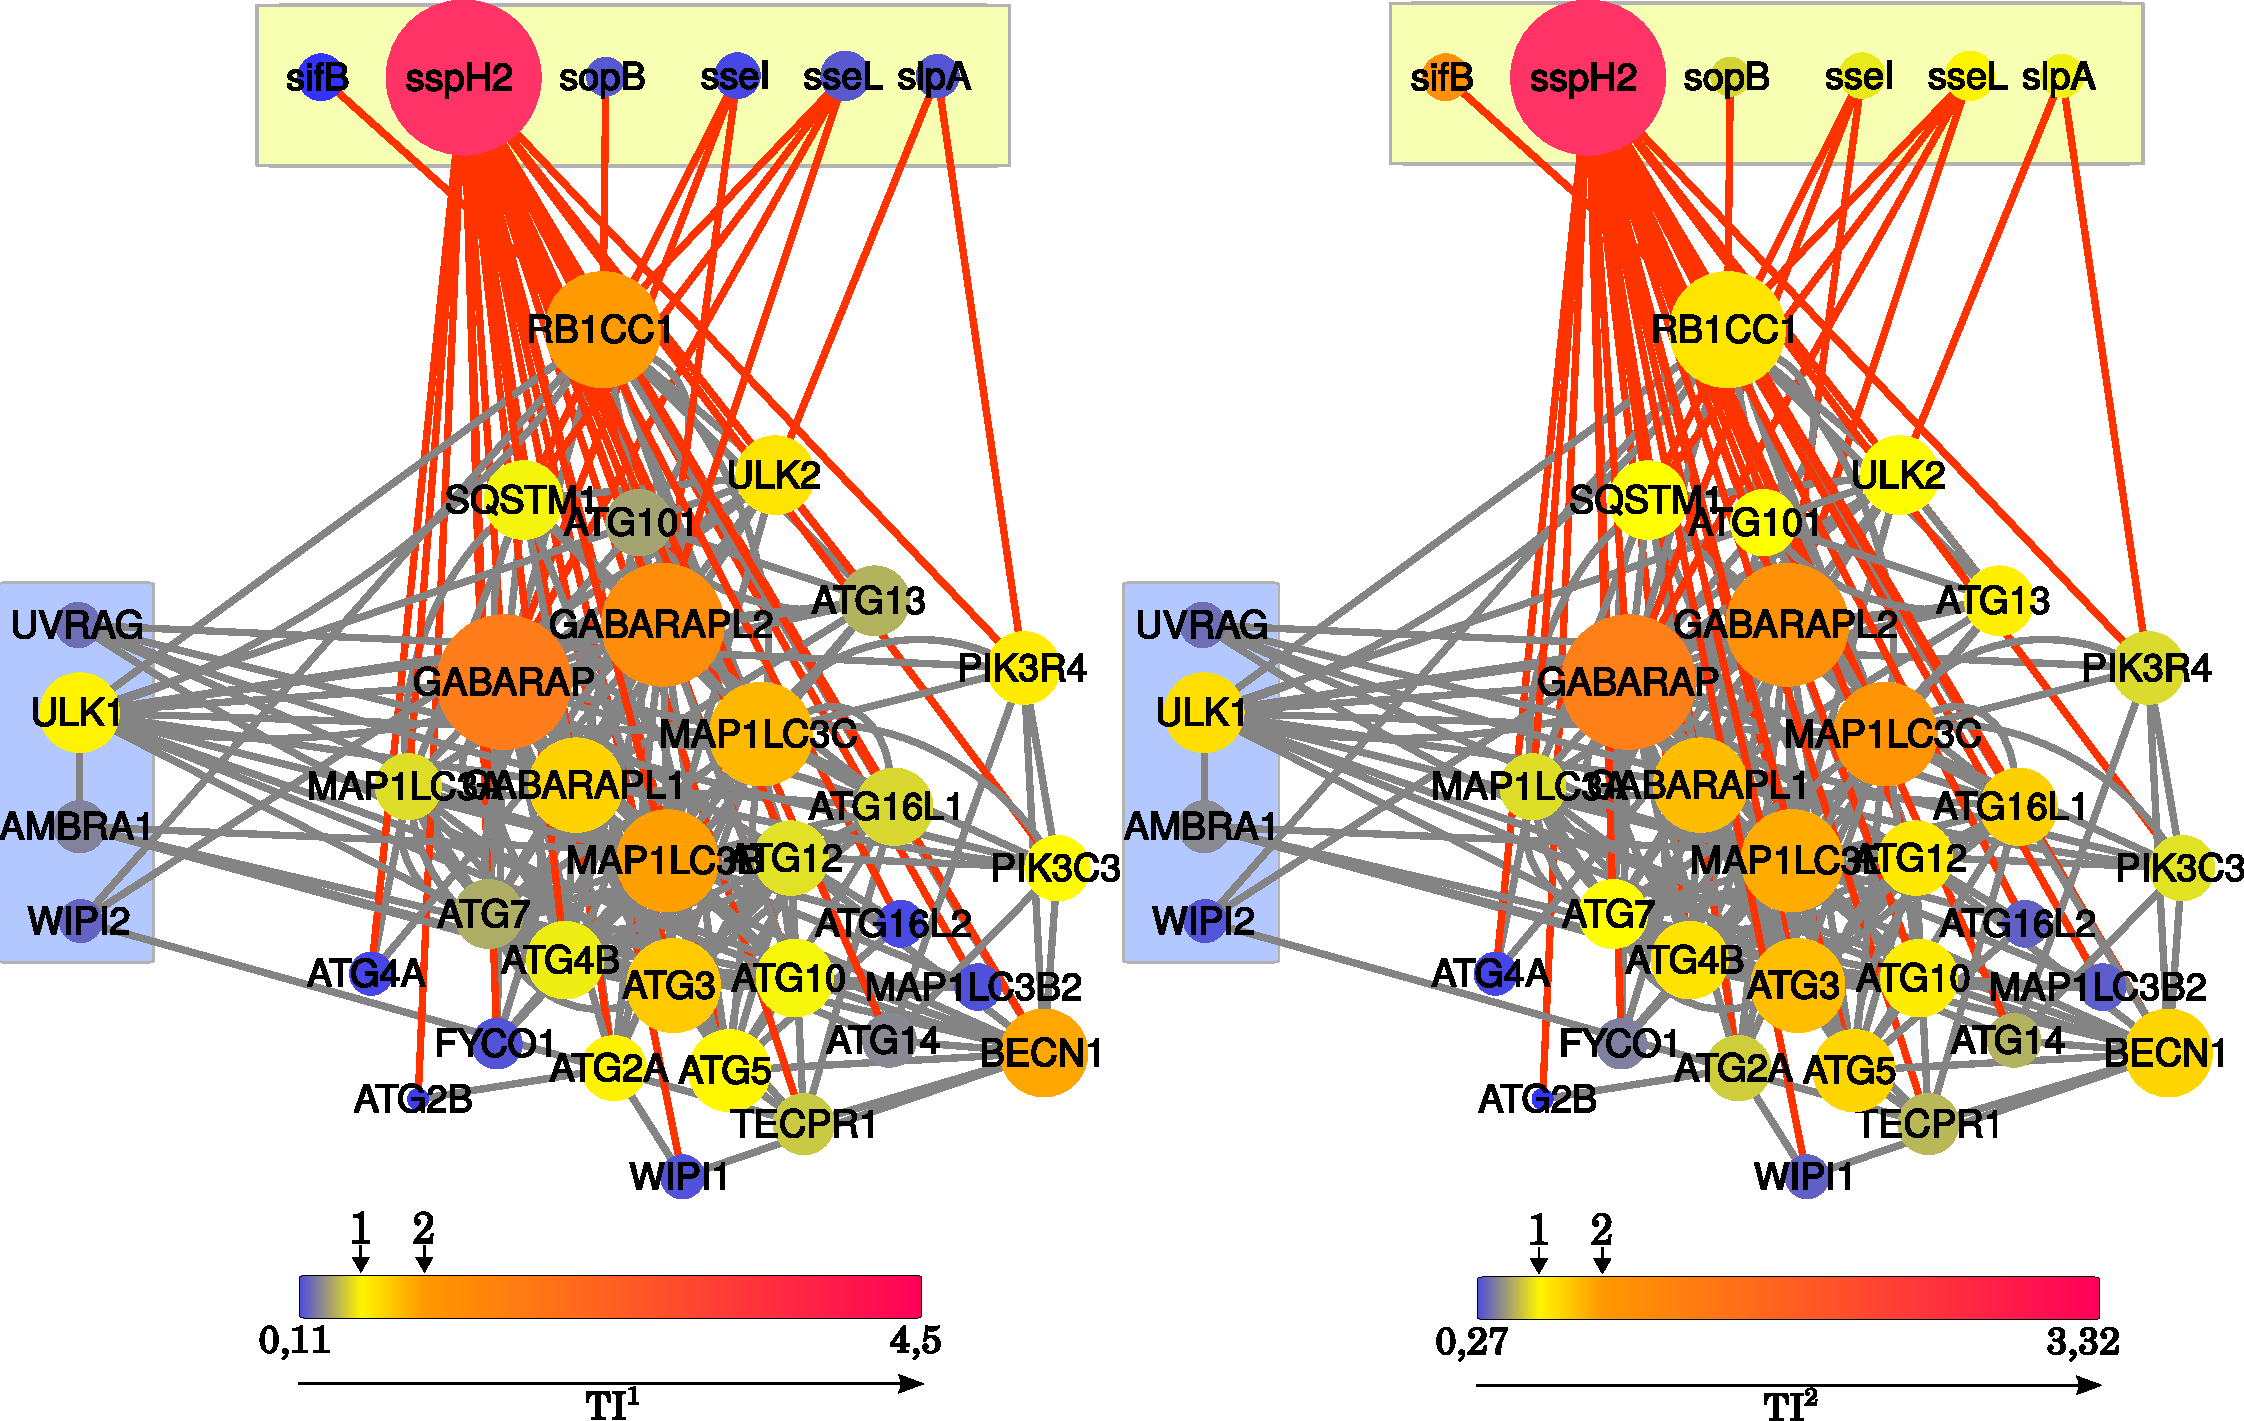
\includegraphics[scale=0.48]{img/connection_prots_v2_complete.pdf}
					\centering
					\caption{ \textbf{Az \textit{ARN} és kapcsolatai az egyesített hálózattal}}		
					\label{fig:connection}
					\begin{imgdesc}
					Az ábrán látható hálózatok az \textit{ARN}-t és a hat \textit{Salmonella} interfész fehérjét ábrázolják. A hálók a TI$^1$ (\textit{felső}) és a TI$^2$ \textit{(alsó)} értékeket szemléltetik. A hálózatok bal oldalán elhelyezkedő kék hátterű pontok jelképezik az \textit{ARN}-nek azon részét, mely csak belső kapcsolatokkal rendelkezik. A hálózatok felső részén elhelyezkedő sárga téglalap tartalmazza a \textit{Salmonet} interfész fehérjéit. A szűkre színű élek a emberi fehérjék közötti kapcsolatok, a narancs színűek pedig a predikciókból származó interspecifikus kapcsolatok. A pontok nagysága arányos a TI értékükkel. A pontok színének megfeleltetése a hálózatok bal alsó részén látható. 
					\end{imgdesc}			 		 
				\end{figure}
		 
		 A \textit{\ref{fig:connection}. ábra} azt is szemlélteti, hogy az interfész fehérjék többsége egy lépésre még nem számít topológiailag erős kölcsönhatónak, viszont két lépésnél már igen. Ennek a jelenségnek az az oka, hogy az interfész fehérjékből viszonylag kevés kapcsolat ered, azonban ezek a kapcsolatok erősen kölcsönható fehérjék. Ezáltal az interfészfehérjékből kiinduló kétlépéses útvonalak erős elsődleges kölcsönhatókon keresztül érik el célpontjukat.
		


				
		\noindent A hat fehérje közül a következő öt bizonyítottan a T3SS-el jut ki a baktériumsejtből, míg az utolsóról kevés információnk van: 
		
		\begin{itemize}
			\item \textbf{sifB} -- A virulencia vagy más néven effektor fehérjék közé tartozik. Fertőzéskor \textit{Salmonella} által kiváltott filamentumok (\textit{Sif}) mentén eltávolodnak az SCV-től (\cite{sifB}). 
			\textit{}
			\item \textbf{sspH2} -- Szintén effektor fehérje. Egy olyan E3 ubikvitin ligáz mely a gazda ubikvitinációs szignalizációját befolyásolja. A szubsztrát hiányában öngátló állapotban van. Szubsztrát kötésekor bekapcsolódik (\cite{ssph2}).  Az sspH2 gátló hatással van az aktin polimerizációra \cite{salmonella_and_host_cell_nature}. 
			
			\item \textbf{sopB} -- Egy olyan esszenciális virulencia fehérje mely inozitol-foszfát-foszfatáz mechanizmusával közvetetten aktiválja a gazda Rho-GTP-ázait. Ilyen kis-G fehérje a Cdc42 és a Rho-G. Az aktiválások hatásának eredője az aktin sejtváz átrendeződése, ami elősegíti a \textit{Salmonella} bejutását a gazdasejtbe \cite{salmonella_and_host_cell_nature}. 
			
			\item \textbf{sseI} -- Egy olyan effektor fehérje melynek aminoterminusa nagy hasonlóságot mutat a SspH2-vel. Filaminon keresztül képes a polimerizált aktin kötésére \cite{salmonella_and_host_cell_nature}. 
			
			\item \textbf{sseL} -- Egy deubikvitináz enzim, mely  mono és polyubikvitin láncok hidrolizálását végzi. Az sseL-nek \textit{in vitro} a lizin-63 kapcsolt ubikvitin láncok sokkal jobb szubsztrátjai, melyből arra lehet következtetni, hogy a proteoszómális degradáció befolyásolása helyett inkább at ubikvitin szignalizáció módosításáért felelős (\cite{sseL}). 
			
			\item \textbf{slpA} -- Ez a fehérje egy peptidil-prolil cisz-transz izomeráz. A szakirodalomban a \textit{Salmonella} ezen fehérjéjéhez nem találtam olyan cikket, mely részletesen leírta volna a funkcióját. Az \textit{Uniprot} adatbázis segítségével azonban találtam a legalább 90\%-os hasonlóságot mutató fehérjék listájában egy \textit{Swissprot} bejegyzést. Ez a hasonló de annotált fehérje az \textit{E. coli} FKBP typusú 16 kDa-os peptidil-prolil izomeráza, mely fehérjék hajtogatási sebességét növeli (\cite{fkbp}).  A két fehérje szekvenciáját az \textit{NCBI BLAST} algoritmusán alapuló \textit{blastp suite-2sequences} és az \textit{ExPASy} fehérjeszekvencia összehasonlító programjával is összehasonlítottam. Az első 92\%-os egyezést adott (E=5$\cdot 10^{-104}$) a második pedig 91,9\%-t.
			
		\end{itemize}
		
		\subsubsection{A T3SS kapcsolatai és a \textit{Salmonella} belső kapcsolatai}
		
		\begin{figure}[H]
			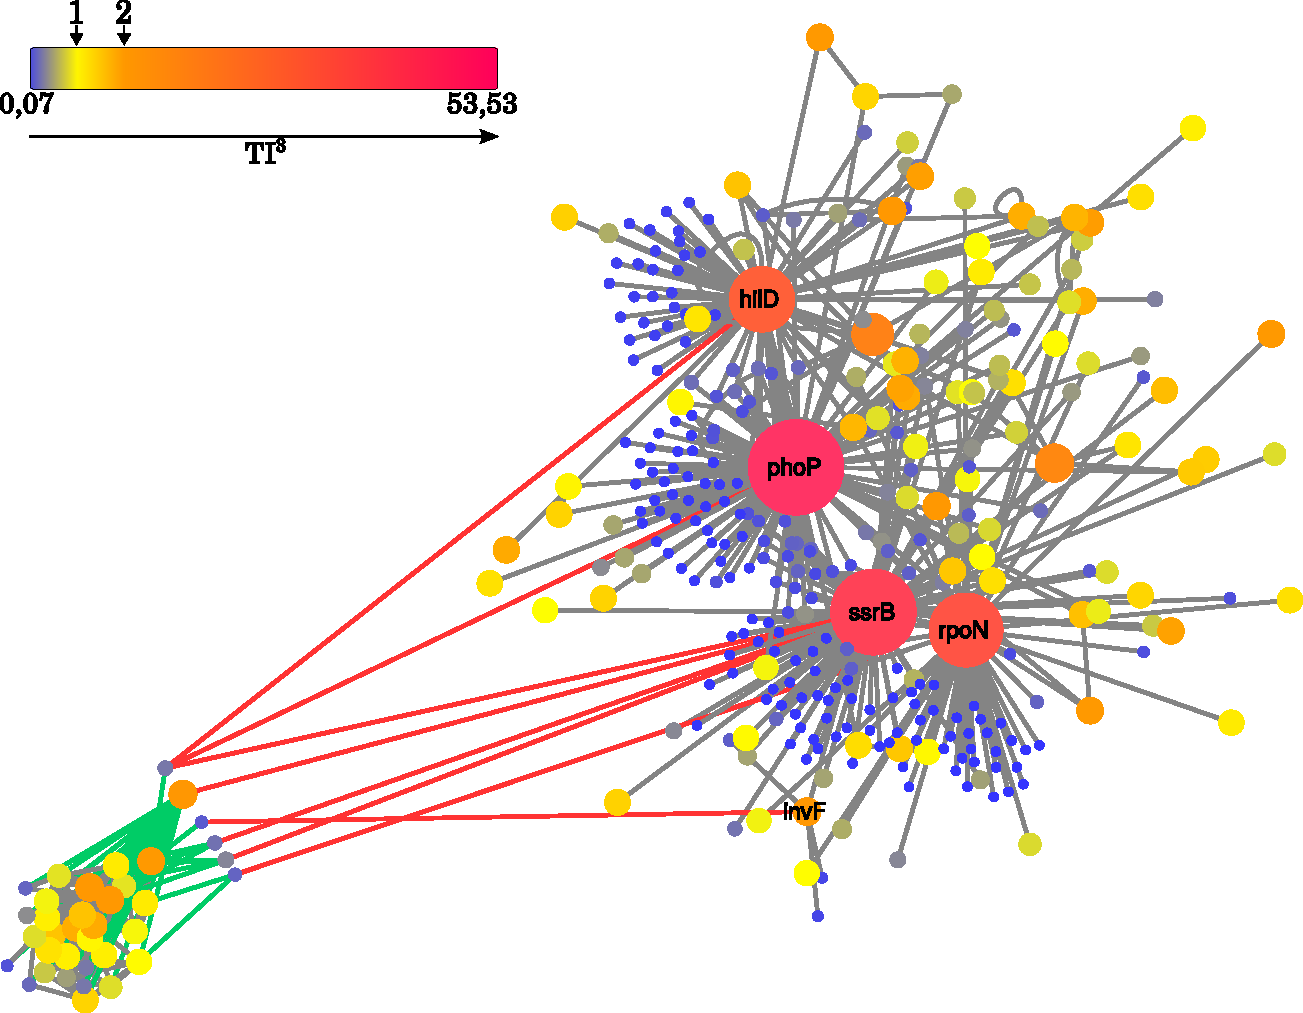
\includegraphics[scale=0.6]{img/t3ss-inner-salmonella.pdf}
			\centering
			\caption{ \textbf{A T3SS fehérjéinek első és második szomszédai}}
			\begin{imgdesc}
				Az ábra a \textit{\ref{fig:merged-3-step}. ábrán} látható hálózatból az interfész fehérjéket valamint ezek első és második szomszédjait tartalmazza. A feltüntetett nevű fehérjék az interfész fehérjék \textit{Salmonella} oldali első szomszédai. A predikciókból származó interspecifikus kapcsolatok zölddel vannak jelölve. Az interfész fehérjéket és \textit{Salmonella}-án belüli első szomszédaikat piros élek kötik össze. A pontok nagysága és színmélysége a TI$^3$ értékükkel arányos. A bal felső sarokban a színeket magyarázó skála látható.
			\end{imgdesc}
			\label{fig:t3ss_inner}			 		 
		\end{figure}

		A \textit{\ref{fig:t3ss_inner}. ábrán} az öt feltüntetett fehérje közül csupán egy az invF olyan amelyik nincs benne se a \textit{\ref{table:merged123}.} se a \textit{\ref{table:salmonet123}. táblázatban}. Így elmondható, hogy a T3SS fehérjék \textit{Salmonella} oldali első szomszédjai a mind a három TI érték szempontból a legmagasabb rangú pontok közé tartoznak.

		\pagebreak
	
\section{Diszkusszió}
		\subsection{Diplomamunkám eredményei}		
		Diplomamunkám során egy humán-\textit{Salmonella} gazda-patogén molekuláris hálózatot készítettem. Ezután a hálózatot egy ökológiai eredetű tisztán topológiai mérőszám a topológiai fontosság (TI) alapján elemeztem. Az index segítségével megpróbáltam felderíteni, hogy melyek a topológiailag fontos fehérjék a humán-\textit{Salmonella} hálózatban és az ezt felépítő két alhálózatban. Emberi oldalról a \textit{Salmonella} autofágiára gyakorolt hatását vizsgáltam. A hálózat előállítása során olyan eszközöket fejlesztettem melyek felhasználhatók hasonló hálózatok építésére és elemzésére. Ezek eszközök segítségével könnyen integrálni lehet a bioinformatikában és rendszer-biológiában használt hálózati formátumokat. A csoportunk által alkalmazott MiTab SQL formátum megkönnyíti a molekuláris hálózati adatok tárolását, átalakítását és elemzését. Az általam írt \textit{PsimiSQL} \textit{Python} osztály megkönnyíti a különböző adatformátumok MiTab SQL-be alakítását. Az általam készített \textit{TopologyAnalyser} \textit{Python} osztály képes a  bármilyen hálózat formátumból könnyen előállítható éllista fájlt topológiai elemzésére.  A csoport által felépített protokoll egy hatékony módszert biztosít molekuláris hálózatok létrehozására. A protokoll jól használhatónak bizonyult \textit{Signalink} és humán-\textit{Salmonella} adatbázis készítésénél.
		
		\subsection{Molekuláris hálózatok jellemzése TI alapján}
		A TI attól függően, hogy milyen lépéshosszra számolják több szempontból is le tudja írni a a vizsgált hálózatot. Az egy lépésre számolt index megmutatja az erős közvetlen kölcsönhatókat. A két lépésre számolt esetben az önhatás és az alakítja a rangsort, hogy a vizsgált pontoknak milyen erős elsődleges kölcsönhatók az első szomszédai. A páros lépésekre számolt TI értékek sokkal jobban függenek az önhatástól, mert mindenképpen tartalmaznak hurkokat. Az egynél hosszabb páratlan útvonalakon alapuló TI értékek pedig a pontok közvetett hatását jellemzik. Bár a páratlan lépéshosszokra számolt TI értékek is tartalmazhatnak hurkokat, de ezek nem az útvonal visszafordulásának eredményei. Az ilyen önhatás, tehát kisebb mértékű és kevésbé közvetlen módon éri el a forrás nódust.
		
		Az általam használt adatszettben a predikciós adatbázisok és a TI együttesen rámutatott egy olyan fehérjére aminek eddig nem írták le a szerepét a \textit{Salmonella} virulenciájában. A TI$^2$ rávilágított a \textit{Salmonella} interfész fehérjéinek fontosságára, amit az irodalom is alátámaszt. Ez abból adódott, hogy az interfész fehérjékből eredő viszonylag kevés kapcsolat erős elsődleges kölcsönhatókon éri el célpontjait. A TI megmutatta azt is hogy az interfész fehérjék első szomszédai nagyon fontosak mind az autofágia, mind a \textit{Salmonella} virulencia és életciklus szabályzásában. Ezzel rávilágítva arra, hogy a \textit{Salmonella} életciklusa erősen függ a gazdával való kölcsönhatásoktól.
		
		A TI bár ökológiai eredetű mérőszám, de képes volt gazda-patogén molekuláris hálózaton a központi molekulák kijelölésére. Az ilyen topológiai mérőszámokat többnyire nem használják molekuláris hálók vizsgálatára. Diplomamunkám rávilágít arra is, hogy biológiailag releváns eredményeket lehet kapni az ilyen mérőszámok molekuláris gazda-patogén hálózatokra alkalmazásával
		
		\subsection{Kitekintések}
		\subsubsection{A TI használata a \textit{Salmonella} és az immunrendszer kölcsönhatásának tanulmányozásához}
		Számtalan forrás \cite{salmonella_and_host_cell_nature} \cite{salmonella_autophagy_nature_old} (\cite{hilD}) említette, hogy a \textit{Salmonella} a bélhámsejtek mellett immunsejtekben, köztük makrofágokban is tud szaporodni. A \textit{Signalink} készítésekor fehérje-fehérje kapcsolatokat integráltam az \textit{InnateDB}-ből. Az \textit{InnateDB} egy kifejezetten immunológiai útvonalakkal foglalkozó publikus rendszer-biológiai adatbázis mely kísérletesen bizonyított jól annotált fehérje-fehérje kapcsolatokat tartalmaz. Az \textit{InnateDB} főleg a veleszületett immunrendszer molekuláris kapcsolataival foglalkozik, melyekből már több mint 18 700 található az a adatbázisban (\cite{innatedb}). Az adatbázis felhasználásával és a TI alkalmazásával meglehetne vizsgálni, hogy a melyek a topológiailag fontos fehérjék az immunrendszer és \textit{Salmonella} kölcsönhatásakor. Egy ilyen hálózat akár új gyógyszercélpontokra is rámutathat.	 
		
 		\subsubsection{A \textit{Salmonella} fertőzés további modellezése}
		A diplomamunkámban csak a TI aspektusában vizsgáltam a gazda-patogén hálózat fehérjéinek fontosságát. Mint a bevezetésben említettem, az ökológiában a kulcs fajok kijelölésére több mérőszámot is használnak egyszerre, melyek más és más aspektusban vizsgálják a fajok fontosságát \cite{jordan_comparison} (\cite{ti}). Érdemes lenne, megvizsgálni azt, hogy más mérőszámok hogyan viselkednek az általam felállított gazda-patogén hálózaton, vagy hogy korrelálnak-e a TI-vel megállapított rangsorral.
 		
 		A szakirodalomban már csináltak másik humán-baktérium gazda-patogén hálózatot, ami inkább a metabolikus megközelítésre fektette a hangsúlyt. A vizsgálatban tüdő makrofágok \textit{Mycobacterium tubercolosis} általi fertőzését modellezték különböző omikai adatok integrálásával készült hálózatban. A teljes genom szintű integrált hoszt-patogén hálózat segítségével metabolikus változásokat modelleztek, melyek segítségével a fertőzést három különböző patológiai fázisra tudták bontani \cite{discussion_alveolar_macrophage}.  Mivel a \textit{Salmonet} is tartalmaz metabolikai adatokat, így az általam összeállított integrált adatbázisban is lehetne hasonló modelleket alkalmazni és ezáltal a fertőzés folyamatának patológiai aspektusaira rávilágítani.
		
		\subsubsection{A TI felhasználása bél mikroökológiájának jellemzésére}
		Mint a bevezetőben említettem, a bél mikrobióta metabolitokkal kommunikál egymással és a humán sejtekkel is. Ilyen mechanizmus a leptin rendszer befolyásolása, vagy a különböző GPCR-ek által például a sejtciklus befolyásolása\cite{buthyrate_immune}.  A bél mikrobióta ilyen módon olyan komoly népegészségügyi betegségekre is hatással van mint az IBD vagy különböző rák típusok\cite{gut_microbiome}.  A bél mikrobióta mindezekre a saját maguk által termelt metabolitokkal is képes hatni \cite{scfa_and_vitamine}. Mivel a \textit{Salmonet} tartalmaz metabolikus kapcsolatokat, így egy jó kiindulási pont lehetne egy bél mikrobióta metabolikus hálózat készítéséhez. Egy ilyen hálózat TI-vel való elemzésével ki lehetne használni a \textit{TI} azon ökológiai aspektusát, hogy a pontok páros lépésszámoknál erősen visszahatnak magukra. Ez életszerű mivel a bél mikrobiótában az egyes baktériumok metabolitjaikkal hatnak más baktériumok anyagcseréjére és így valószínűleg azok biomasszájára is \cite{gut_microbiome}.  Egy ilyen a TI-n alapuló rangsorban ki lehetne jelölni hogy a meta-omikák által megállapított személyre jutó körülbelül 160 domináns baktérium fajból \cite{meta_omics} melyek azok amelyek úgymond kulcsfajként viselkednek. Gyógyászati szempontból meg lehetne nézni a különbséget a topológiailag legfontosabb kulcs baktérium fajok között egészséges és például Crohn betegségben, vagy rákban szenvedő személyek mikrobiótája között. Hasonló vizsgálatokkal a gazda-patogén szempont mellett akár a mutualisztikus kapcsolatokat is vizsgálni lehetne humán-bélbaktérium, vagy bélmikróbióta baktérium-baktérium hálózatokban.
		

		\subsubsection{A modellekből nyert adatok kísérletes ellenőrzésének lehetősége}
		Az eddig felsorolt kitekintések és alkalmazási lehetőséget többnyire új elméleti módszerekre világítottak rá, melyek kísérletes ellenőrzése meglehetősen nehézkes. Azonban organoidok segítségével lehetőség lenne a legtöbb eddig felsorolt elméleti vizsgálat \textit{in vitro} ellenőrzésére. Az organoidokon végzett vizsgálatok már eddig is sok információval szolgáltak az organogenezis, a regeneratív orvoslás a tumorigenezis és az emésztőrendszer működésével kapcsolatban. Az organoidok egyetlen izolált szöveti őssejtből előállított, a valódi \textit{in vivo} szövet karakterisztikáit tükröző mesterségesen \textit{in vitro} struktúrák (\cite{organoid}).
		Egér bélből állítottak elő olyan organoidokat melyek tükrözték a a bél lumen szerkezetét, ezekben kriptákat határoló kitüremkedések voltak megfigyelhetők. Az ilyen módon előállított szérum nélkül, csupán szöveti niche faktorokkal kezelt organoidok önfenntartók és akár több mint egy évig életben maradnak (\cite{organoid}).  Ilyen rendszerekben lehetőség nyílik a rendszer-biológiai modellekből és fontossági listákból nyert elméleti eredmények, jóslatok kísérleti ellenőrzésére.
		
		\subsubsection{A TI alkalmazásának lehetősége a botanikában}
		Az eddig említett elméleti és gyakorlati lehetőségek mind valamilyen szinten humán relevanciával rendelkeztek. Azonban bél mikrobiomhoz hasonlóan a növények is komplex mikrobiológiai rendszerben élnek, melyben mikrobák széles skálája fordul elő. 
		A hasonlóan az állati immunrendszerhez a növények is felismerik a patogén mintázatot és specifikus válaszokat adnak rá. A növényi fertőzésekor kis molekulák széles skálája vesz részt a védekezésben. Ezek a molekulák között egymás erősítő és gátló hatások figyelhetőek meg. A növényi patogének hasonló molekulákkal próbálják a fitohormon homeosztázist módosítani \cite{discussion_plant_network} . Az ilyen adatokból épített molekuláris hálózatok elemzése jó alapot szolgáltathat a mezőgazdaságilag fontos növények és patogénjeik között fellépő mechanizmusok feltérképezéséhez.
		
		\pagebreak

\section{Összefoglalás}
		
		Diplomamunkám során olyan eszközöket hoztam létre melyek megkönnyítik a molekuláris hálózatok építését.  Az általunk tervezett \textit{MiTab SQL} formátum megkönnyíti a molekuláris hálózat adatok tárolását, átalakítását és elemzését. Létrehoztam a  \textit{PsimiSQL Python} osztályt, melynek segítségével számos különböző formátumú adat gyorsan átalakítható \textit{MiTab SQL} formátumra. A kutatócsoportunk létrehozott egy olyan protokollt, mely hatékony módszert biztosít molekuláris hálózatok létrehozására. A protokoll segítségével hatékonyan fel tudtam építeni az ember-\textit{Salmonella} adatbázist.
		
		\vspace{22pt}
		
		A \textit{TopologyAnalyser} egy szintén általam készített \textit{Python} oszály mely segítségével él-lista fájlok elemezhetők. Az osztály képes a beadott hálózat TI értékeinek kiszámítására. Ilyen él-listák bármilyen hálózatból könnyen készíthetők. 
		
		\vspace{22pt}
		
		A TI-t én alkalmaztam először gazda patogén molekuláris hálózaton. A TI alkalmasnak bizonyult Bár a TI egy ökológiai mérőszám, de mégis használhatónak bizonyult a gazda-patogén hálózat központ fehérjéinek kijelölésében. Az ilyen típusú topológiai mérőszámokat csak ritkán alkalmazzák molekuláris hálózatokra. A diplomamunkám bebizonyította, hogy biológiailag releváns eredmények érhetőek el az ilyen mérőszámok alkalmazásával.

		\vspace{22pt} 
		
		Az integrált adatbázisban az ember-\textit{Salmonella} predikciók és a TI kiemelt egy olyan fehérjét aminek \textit{Salmonella} virulenciájában játszott szerepe még nincsen leírva.

		\vspace{22pt}
		
		Az általam készített adatszerkezetek és szkriptek segítségével meghatározott TI alapján a \textit{Salmonella} és bélsejtek közti kapcsolatokat vizsgáló kísérletek már folyamatban vannak.
		
		
		\pagebreak
		
		

\section{Summary}
		
		In my thesis work I created efficient tools and data structures that can be used for building molecular networks. Our \textit{MiTab SQLite} format makes it easier to  store, transform and analyze molecular network data. I built the \textit{PsimiSQL Python} class that can be used to convert several data formats to MiTab SQL easily. Our research group created a powerful protocol for constructing molecular networks. The protocol proved to be well usable for the establishment of the human-\textit{Salmonella} database.
		
		\vspace{22pt}
		
		I also built another \textit{Python class} \textit{TopologyAnalyser} that can analyze edge-list files. The class can count the TI values forthe given network. Edge-list files can be easily obtained from any network. 
		
		\vspace{22pt}
		
		For the first time I applied TI in the analysis of a host-pathogen molecular network. Although the topological importance is an ecological index, it is proven that it can be used to mark the central proteins of a host-pathogen network. These kind of topological indices are rarely used for the analysis of molecular networks. My thesis reveals that biologically relevant results can be obtained by using indices like this.
		
		\vspace{22pt} 
		
		In this data set, the predictions and the topological importance marked a protein that haven't been described in \textit{Salmonella} virulence yet.
		 
		\vspace{22pt} 
		
		Experiments that aim to explore the connections between \textit{Salmonella} and enterocytes have already started based on results that were achieved by my scripts and data structures.
				
		\pagebreak

\section{Köszönetnyilvánítás}

Ezúton szeretném megragadni az alkalmat arra, hogy köszönetemet és tiszteletemet
fejezzem ki mindenkinek, aki a szakdolgozatom elkészítéséhez nagyban hozzájárult.


Köszönetet szeretnék mondani kiváló szakmai tanácsaiért és állandó segítőkészségéért témavezetőmnek Kadlecsik Tamásnak.

Köszönetet szeretnék mondani tudományos tanácsaiért, diplomamunkám irányításáért valamint szakdolgozatom szakmai és stilisztikai javításáért témavezetőmnek Korcsmáros Tamásnak.

Dolgozatom tudományos és stilisztikai anyagának folyamatos figyelemmel
követéséért, javításáért és építő javaslataiért szeretnék köszönetet kifejezni Fazekas Dávidnak.

Tanácsaikért és figyelmükért szeretnék köszönetet mondani az Netbiol kutatócsoport
munkatársainak.

Végül, de nem utolsó sorban szeretném kifejezni megbecsülésemet, köszönetemet
családtagjaimnak és barátaimnak, akik szeretetükkel és segítségükkel mindvégig támaszt
nyújtottak ELTE-s és az azt megelőző tanulmányaim során, és szakdolgozatom
elkészítésének teljes ideje alatt türelmet tanúsítottak irántam, illetve igyekeztek nyugodt
környezetet biztosítani a tudományos anyag feldolgozása közben! Köszönöm!

\pagebreak

\section{Nyilatkozat}

Név: Horváth Balázs

\noindent Neptun azonosító: X6YDH1

\noindent ELTE Természettudományi Kar, biológus mesterszak

\noindent Diplomamunka címe: \textit{Bakteriális patogén és ember közötti molekuláris hálózatok vizsgálata}

\vspace{32pt}

A diplomamunka szerzőjeként fegyelmi felelősségem tudatában kijelentem, hogy a
dolgozatom önálló munkám eredménye, saját szellemi termékem, abban a
hivatkozások és idézések standard szabályait következetesen alkalmaztam.
Tudomásul veszem, hogy plágiumnak számít:
\begin{itemize}
	\item szó szerinti idézet közlése idézőjel és hivatkozás megjelölése nélkül;
	\item tartalmi hivatkozás a forrás megjelölése nélkül;
	\item más személy publikált gondolatainak saját gondolatként való feltüntetése.
\end{itemize}

Kijelentem továbbá, hogy a szakdolgozat leadott nyomtatott példányai és elektronikus
változata szövegükben, tartalmukban megegyeznek.

\vspace{32pt}

\begin{center}
\begin{tabular}{clc}
Budapest, 2016. május 13. & \hspace{32pt} & \par\noindent\makebox[2.5in]{\hrulefill} \\
                          & \hspace{32pt} & \textit{a hallgató aláírása}                  
\end{tabular}
\end{center}



\pagebreak


\printbibliography[title={Felhasznált irodalom},heading=bibintoc,type=article]

\printbibliography[title={Internetes hivatkozások},heading=bibintoc,type=misc]

\end{document}

